\def\year{2021}\relax
%File: formatting-instructions-latex-2021.tex
%release 2021.2
\documentclass[letterpaper]{article} % DO NOT CHANGE THIS
\usepackage{aaai21}  % DO NOT CHANGE THIS
\usepackage{times}  % DO NOT CHANGE THIS
\usepackage{helvet} % DO NOT CHANGE THIS
\usepackage{courier}  % DO NOT CHANGE THIS
\usepackage[hyphens]{url}  % DO NOT CHANGE THIS
\usepackage{multirow}
\usepackage{amsmath}
% \usepackage{breqn}
\usepackage{bm}
\usepackage{graphicx} % DO NOT CHANGE THIS
\urlstyle{rm} % DO NOT CHANGE THIS
\def\UrlFont{\rm}  % DO NOT CHANGE THIS
\usepackage{natbib}  % DO NOT CHANGE THIS AND DO NOT ADD ANY OPTIONS TO IT
\usepackage{caption} % DO NOT CHANGE THIS AND DO NOT ADD ANY OPTIONS TO IT
\usepackage{booktabs}

\frenchspacing  % DO NOT CHANGE THIS
\setlength{\pdfpagewidth}{8.5in}  % DO NOT CHANGE THIS
\setlength{\pdfpageheight}{11in}  % DO NOT CHANGE THIS
\newcommand*{\affaddr}[1]{#1} % No op here. Customize it for different styles.
\newcommand*{\affmark}[1][*]{\textsuperscript{#1}}
\newcommand*{\email}[1]{\texttt{#1}}
\nocopyright
%PDF Info Is REQUIRED.
% For /Author, add all authors within the parentheses, separated by commas. No accents or commands.
% For /Title, add Title in Mixed Case. No accents or commands. Retain the parentheses.
\pdfinfo{
/Title (AAAI Press Formatting Instructions for Authors Using LaTeX -- A Guide)
/Author (AAAI Press Staff, Pater Patel Schneider, Sunil Issar, J. Scott Penberthy, George Ferguson, Hans Guesgen, Francisco Cruz, Marc Pujol-Gonzalez)
/TemplateVersion (2021.2)
} %Leave this
% /Title ()
% Put your actual complete title (no codes, scripts, shortcuts, or LaTeX commands) within the parentheses in mixed case
% Leave the space between \Title and the beginning parenthesis alone
% /Author ()
% Put your actual complete list of authors (no codes, scripts, shortcuts, or LaTeX commands) within the parentheses in mixed case.
% Each author should be only by a comma. If the name contains accents, remove them. If there are any LaTeX commands,
% remove them.

% DISALLOWED PACKAGES
% \usepackage{authblk} -- This package is specifically forbidden
% \usepackage{balance} -- This package is specifically forbidden
% \usepackage{color (if used in text)
% \usepackage{CJK} -- This package is specifically forbidden
% \usepackage{float} -- This package is specifically forbidden
% \usepackage{flushend} -- This package is specifically forbidden
% \usepackage{fontenc} -- This package is specifically forbidden
% \usepackage{fullpage} -- This package is specifically forbidden
% \usepackage{geometry} -- This package is specifically forbidden
% \usepackage{grffile} -- This package is specifically forbidden
% \usepackage{hyperref} -- This package is specifically forbidden
% \usepackage{navigator} -- This package is specifically forbidden
% (or any other package that embeds links such as navigator or hyperref)
% \indentfirst} -- This package is specifically forbidden
% \layout} -- This package is specifically forbidden
% \multicol} -- This package is specifically forbidden
% \nameref} -- This package is specifically forbidden
% \usepackage{savetrees} -- This package is specifically forbidden
% \usepackage{setspace} -- This package is specifically forbidden
% \usepackage{stfloats} -- This package is specifically forbidden
% \usepackage{tabu} -- This package is specifically forbidden
% \usepackage{titlesec} -- This package is specifically forbidden
% \usepackage{tocbibind} -- This package is specifically forbidden
% \usepackage{ulem} -- This package is specifically forbidden
% \usepackage{wrapfig} -- This package is specifically forbidden
% DISALLOWED COMMANDS
% \nocopyright -- Your paper will not be published if you use this command
% \addtolength -- This command may not be used
% \balance -- This command may not be used
% \baselinestretch -- Your paper will not be published if you use this command
% \clearpage -- No page breaks of any kind may be used for the final version of your paper
% \columnsep -- This command may not be used
% \newpage -- No page breaks of any kind may be used for the final version of your paper
% \pagebreak -- No page breaks of any kind may be used for the final version of your paperr
% \pagestyle -- This command may not be used
% \tiny -- This is not an acceptable font size.
% \vspace{- -- No negative value may be used in proximity of a caption, figure, table, section, subsection, subsubsection, or reference
% \vskip{- -- No negative value may be used to alter spacing above or below a caption, figure, table, section, subsection, subsubsection, or reference

\setcounter{secnumdepth}{0} %May be changed to 1 or 2 if section numbers are desired.

% The file aaai21.sty is the style file for AAAI Press
% proceedings, working notes, and technical reports.
%

% Title

% Your title must be in mixed case, not sentence case.
% That means all verbs (including short verbs like be, is, using,and go),
% nouns, adverbs, adjectives should be capitalized, including both words in hyphenated terms, while
% articles, conjunctions, and prepositions are lower case unless they
% directly follow a colon or long dash


\title{Graph-based Multi-hop Reasoning for Long Text Generation}

%  common sense  skeleton  
%  concept level coherence
% \author{
% Liang Zhao\affmark[1]\thanks{\ \ Equal Contribution.}, \ 
% Jingjing Xu\affmark[2]\footnotemark[1], \ 
% Junyang Lin\affmark[3], \ 
% Yichang Zhang\affmark[3], \ 
% Hongxia Yang\affmark[3],  \
% Xu Sun\affmark[1,2]
% \\ 
% \affmark[1] Center for Data Science, Beijing Institute of Big Data Research, Peking University \\
% \affmark[2] MOE Key Lab of Computational Linguistics, School of EECS, Peking University  \\
% \affmark[3] Alibaba Group    \\
% \email{\{zhao1iang,jingjingxu,xusun\}@pku.edu.cn }\\
% \email{\{junyang.ljy,yichang.zhang,yang.yhx\}@alibaba-inc.com }\\
% }
\author{
Liang Zhao\thanks{\ \ Equal Contribution.}, \textsuperscript{\rm 1} 
Jingjing Xu\footnotemark[1], \textsuperscript{\rm 2} 
Junyang Lin, \textsuperscript{\rm 3} 
Yichang Zhang, \textsuperscript{\rm 3} 
Hongxia Yang, \textsuperscript{\rm 3} 
Xu Sun, \textsuperscript{\rm 1,2} \\
}
\affiliations{
\textsuperscript{\rm 1} Center for Data Science, Beijing Institute of Big Data Research, Peking University \\
\textsuperscript{\rm 2} MOE Key Lab of Computational Linguistics, School of EECS, Peking University \\
\textsuperscript{\rm 3} Alibaba Group \\
\{zhao1iang,jingjingxu,xusun\}@pku.edu.cn, \{junyang.ljy,yichang.zyc,yang.yhx\}@alibaba-inc.com
}


\begin{document}

\maketitle

\begin{abstract}
Long text generation is an important but challenging task. 
The main problem lies in learning sentence-level semantic dependencies which traditional generative models often suffer from. 
To address this problem, we propose a
% \textbf{Multi-hop Reasoning based Generative (MRG)}
\textbf{Multi-hop Reasoning Generation (MRG)} approach that
 incorporates multi-hop reasoning over a knowledge graph to learn semantic dependencies among sentences. MRG consists of two parts, a graph-based multi-hop reasoning module and a path-aware sentence realization module. The reasoning module is responsible for 
%  searching skeleton paths from a knowledge graph 
% searching paths from a knowledge graph as a skeleton 
searching skeleton paths from a knowledge graph
 to imitate the imagination process in the human writing for semantic transfer. Based on the inferred paths, the sentence realization module then generates a complete sentence. 
%  Owing to the lack of human annotation, 
%  we adopt a self-supervised approach to construct  pseudo parallel corpus 
%  to train the modules.
%  the lack of human-annotated training corpus, 
%  supervisory signals 
 Unlike previous black-box models, MRG explicitly infers the skeleton path, which provides explanatory views to understand how the proposed model works.  
We conduct experiments on three representative tasks, including story generation, review generation, and product description generation.
%  Both automatic and human evaluation demonstrate the effectiveness of the proposed model. The proposed model outperforms strong baselines significantly, especially in terms of informativeness, diversity and coherence.   
 Automatic and manual evaluation show that
our proposed method can generate more informative and coherent long text than
strong baselines, such as pre-trained models (e.g. GPT-2) and knowledge-enhanced models. 
% Our analyses demonstrate the inferred skeleton paths can efficiently build semantic dependencies among sentences and provide explanatory views to understand the generation process.
%Long text generation is an important but challenging task. The challenge lies within how to efficiently learn semantic dependencies among sentences. Here we introduce a \textbf{multi-hop Reasoning Generation (MRG)} approach that can  perform  multi-hop reasoning in knowledge graph to model the complex semantic relation between sentence to generate and the context and provide explanatory reasoning path for long text generation.
% The key idea is to model the reasoning process during writing like human being. 
%MRG can efficiently explore useful reasoning path for text generation with a self-supervised way, even there exists no  high-quality artificial knowledge graph.  With the help of the semantic relationship established by the reasoning path among sentences in knowledge graph, our approach can generate more coherent and informative long text. 

\end{abstract}

\section{Introduction}
% point out the importance , such as entertainment, e-commerce, and so on is an important but challenging task and is applicable in a number of fields. It

Long text generation is an important task and is applicable in a number of fields. It requires a model to generate a coherent and informative long text sequence which consists of several sentences based on free-format source text, such as a table, a topic sentence, or even some keywords~\cite{regina-et-al:table2text,nm:story_generation_2006,feng-et-al:2018topic}. 
% Long text generation techniques provide an automatic way to generate a large amount of high-quality contents, which can improve the efficiency of human writing. 
Recently, these techniques have been applied to many real-world tasks, like automatic story generation~\cite{nm:story_generation_2006}, review generation~\cite{reviewe-generation} as well as product description generation \cite{chen-et-al:product_description_generation}. %Since long text generation has great potential in application, it has become one of the focuses in both research and industry.
% and recent technology development in deep learning has made the generation of long text more possible than ever
% a simple definition
% Long text generation aims at generating coherent and cohesive long text with multiple sentences, such as story \cite{nm:story_generation_2006}, review \cite{edmund-et-al:wong2013autocomment}, and essay \cite{feng-et-al:2018topic}. 

% To be more specific, an automatic long text generation system is required to generate a meaningful coherent and informative long text based on several keywords or a topic sentence. 
% an automatic natural language generation system is required to generate a meaningful long  text based on the given information, such as keywords or a topic sentence. 
% of a story and the basic information of an item. 
% The sentences that it generates should be related to the input information and mutually connected on multiple aspects, including syntax, semantics and pragmatics. 

% are either a conditional language model \cite{gpt2} or a model with the sequence-to-sequence framework \cite{Seq2Seq,Transformer}. They 

\begin{figure}[t] 
\centering
\footnotesize
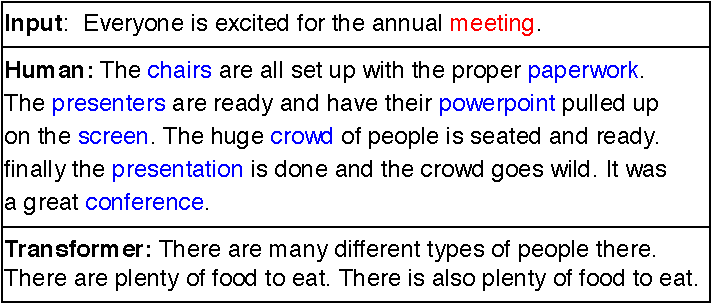
\includegraphics[width=1.0\linewidth]{intro_example.pdf}
% \includegraphics[\linewidth]{graph_trans.pdf}
\caption{The comparison between stories generated by a human and a widely-used generative model Transformer. As shown in the example, human can create diverse and coherent sentences with their imagination. For illustration, we highlight several skeleton words important for sentence-level semantic dependencies. In contrast, the machine-generated text is boring and repetitive. % Red word is concept in input through which humans imagine a lot of related concepts (blue words) for text generation. In contrast, machine-generated (transformer) text is boring and repetitive due to lack of imagination 
\label{fig:intro_example}}
\end{figure}


%Most of the current models have little power to model such dependencies.
Long text generation is more challenging than single sentence generation~\cite{langkilde-et-al:sentece_generation} in that it requires a model to learn the sentence-level semantic dependencies. Compared with word-level semantic dependencies in a single sentence,
% with short distance
sentence-level semantic dependencies are a kind of long-distance dependency that are harder to learn. 
Current end-to-end generative models~\citep{sutskever-et-al:seq2seq,vaswani-et-al:transformer} often adopt an attention mechanism to model the context dependencies, which fuses all word information together to generate the next word in a weighting way. 
Despite promising results in single sentence generation, these models suffer from complicated and sparse dependencies in long text generation with much longer contexts. Such dependencies make models hard to learn sufficient knowledge to infer semantic transfer among sentences.  Thus, these models tend to generate repetitive and boring sentences like a context-free language model, as shown in Figure~\ref{fig:intro_example}. In comparison, human can write diverse texts with coherent semantic transfer among sentences with their imagination. % about how new concepts can be transferred from  previously generated concepts, which current end-to-end generative models have not learned well.
Imagination is said to be a part of literacy process and it highly contributes to writing \citep{colello:colello2007imagination}.
% % They tend to generate repetitive and general sentences.     as they inherently learn relatively simple patterns of texts only via attention mechanism, suffering from repetitive and general text.
% and model semantic dependencies via attention mechanism which only extracts and utilizes  internal information.
% their attention mechanism 
% only extracts and utilizes the conceptual information from source side without considering the behind conceptual realtion . 
% Sentence-level semantic dependencies in human-writing text usually are built by imagination about concepts which can be formulated as
%Sentence-level semantic dependencies in human-writing text usually are built by imagination about how can concepts in context extend to concepts in subsequent sentences.
% the imagination process is the semantic dependencies building process.
% Apparently such model architectures cannot make use of the external knowledge, let alone performing reasoning.
% For example, in story generation task, 
% For example, in story generation task, topic sentence and sentences to generate are ``Last week I attended a wedding for the first time'' and  ``..., Bride and guests dance together in church to celebrate this wonderful moment'' , respectively. Therefore, model need to model the semantic dependencies via some concepts in topic sentence``wedding'' and concepts in target sentence  such as ``bride'', ``dance'' ``church'' and ``celebrate''. 
%Specifically, a human-writing sentence usually contains multiple concepts and the concept path bridging concepts in different sentences can be regarded as such semantic connection. 
%Semantic connection between concepts can be modeled in a  knowledge graphs.
% So the model how to transfer between concepts to establish a semantic connection.
%Inside a knowledge graph, it is common that concepts are not directly connected but instead connected with multiple intermediate nodes.  Therefore, it is necessary that a model 
%should have the ability of conducting multi-hop reasoning in order to connect related concepts for the generation of more coherent and cohesive texts. 

% Essentially, this task can be defined as a text-to-text problem, and sequence-to-sequence model, such as the conventional attention-based Seq2Seq model \cite{Seq2Seq, attention} and the recent Transformer \cite{Transformer} which has achieved great success in a series of natural language generation tasks, can perform such text generation. However, most of the current natural language generation models focus on generating short texts(less than 20 words or just one sentence). Yet long text generation is more challenging compared with short text generation. It requires the generated sentences to be semantically cohesive.   
% To reach this goal, the model should has the capacity to learn complex semantic dependencies among sentence.
% % and perform reasoning while generating sentences so that it can build a semantic connection with the context. 



% Most of the current generation models are either a conditional language model or a model with the sequence-to-sequence framework. They have little power to model the conceptual reasoning between sentences as they inherently learn relatively simple patterns of texts and their attention mechanism only extracts and utilizes the internal information. Apparently such model architectures cannot make use of the external knowledge, let alone performing reasoning.

% Most of the current generation models are either a conditional language model or a model with the sequence-to-sequence framework.

% Essentially, this task can be defined as a text-to-text problem, and sequence-to-sequence model, such as the conventional attention-based Seq2Seq model \cite{Seq2Seq, attention} and the recent Transformer \cite{Transformer} which has achieved great success in a series of natural language generation tasks, can perform such text generation. However, most of the current natural language generation models focus on generating short texts(less than 20 words or just one sentence). Yet long text generation is more challenging compared with short text generation. It requires the generated sentences to be semantically cohesive.   
% To reach this goal, the model should has the capacity to learn complex semantic dependencies among sentence.
% % and perform reasoning while generating sentences so that it can build a semantic connection with the context. 
% Specifically, a sentence usually contains multiple concepts and the concept path bridging concepts in different sentences can be regarded as such semantic connection. Inside a knowledge graph, it is common that concepts are not directly connected but instead connected with multiple intermediate nodes. 
% Therefore, it is necessary that a model should have the ability of multi-hop reasoning in order to connect related concepts for the generation of more coherent and cohesive texts.


% Most of the current generation models are either a conditional language model or a model with the sequence-to-sequence framework. They have little power to model the conceptual reasoning between sentences as they inherently learn relatively simple patterns of texts and their attention mechanism only extracts and utilizes the internal information. Apparently such model architectures cannot make use of the external knowledge, let alone performing reasoning.

% Essentially, this task can be defined as a text-to-text problem, and sequence-to-sequence model, such as the conventional attention-based Seq2Seq model \cite{Seq2Seq, attention} and the recent Transformer \cite{Transformer} which has achieved great success in a series of natural language generation tasks, can perform such text generation. However, most of the current natural language generation models focus on generating short texts(less than 20 words or just one sentence). Yet long text generation is more challenging compared with short text generation. It requires the generated sentences to be semantically cohesive.   
% To reach this goal, the model should has the capacity to learn complex semantic dependencies among sentence.
% % and perform reasoning while generating sentences so that it can build a semantic connection with the context. 
% Specifically, a sentence usually contains multiple concepts and the concept path bridging concepts in different sentences can be regarded as such semantic connection. Inside a knowledge graph, it is common that concepts are not directly connected but instead connected with multiple intermediate nodes. 
% Therefore, it is necessary that a model should have the ability of multi-hop reasoning in order to connect related concepts for the generation of more coherent and cohesive texts.

% Long text generation is an important task for natural language generation and it is applicable in a number of fields, including entertainment and e-commerce. Recently, it has been applied to automatic story generation \cite{nm:story_generation_2006}, review generation as well as product description generation \cite{edmund-et-al:wong2013autocomment,feng-et-al:2018topic,chen-et-al:product_description_generation}. It is able to provide readers with a large amount of their required and preferred contents without the engagement of human, which can highly improve the efficiency of content generation in many industries. As this task has great potential and value in application, and recent technology development in deep learning and natural language processing has made the generation of high-quality long text more possible than ever, this task has become one of the focuses in both research and industry.

% % a simple definition
% % Long text generation aims at generating coherent and cohesive long text with multiple sentences, such as story \cite{nm:story_generation_2006}, review \cite{edmund-et-al:wong2013autocomment}, and essay \cite{feng-et-al:2018topic}. 

% To be more specific, an automatic long text generation system is required to generate a meaningful coherent and informative long text based on several keywords or a topic sentence.
% % an automatic natural language generation system is required to generate a meaningful long  text based on the given information, such as keywords or a topic sentence.
% % of a story and the basic information of an item. 
% % The sentences that it generates should be related to the input information and mutually connected on multiple aspects, including syntax, semantics and pragmatics.
% Essentially, this task can be defined as a text-to-text problem, and sequence-to-sequence model, such as the conventional attention-based Seq2Seq model \cite{Seq2Seq, attention} and the recent Transformer \cite{Transformer} which has achieved great success in a series of natural language generation tasks, can perform such text generation.
% There are increasing attention drawn by this area due to their great potential application value in reality.   Despite its great application value, most of the recently neural generative model focused on generating single and short sentence
% \cite{Seq2Seq,autoencoder,seqgan,pixelrnn,Transformer}, such as machine translation and response generation,  generating paragraph-level long text  has been less explored.
% \begin{figure}[t] 
% \centering
% \footnotesize
% 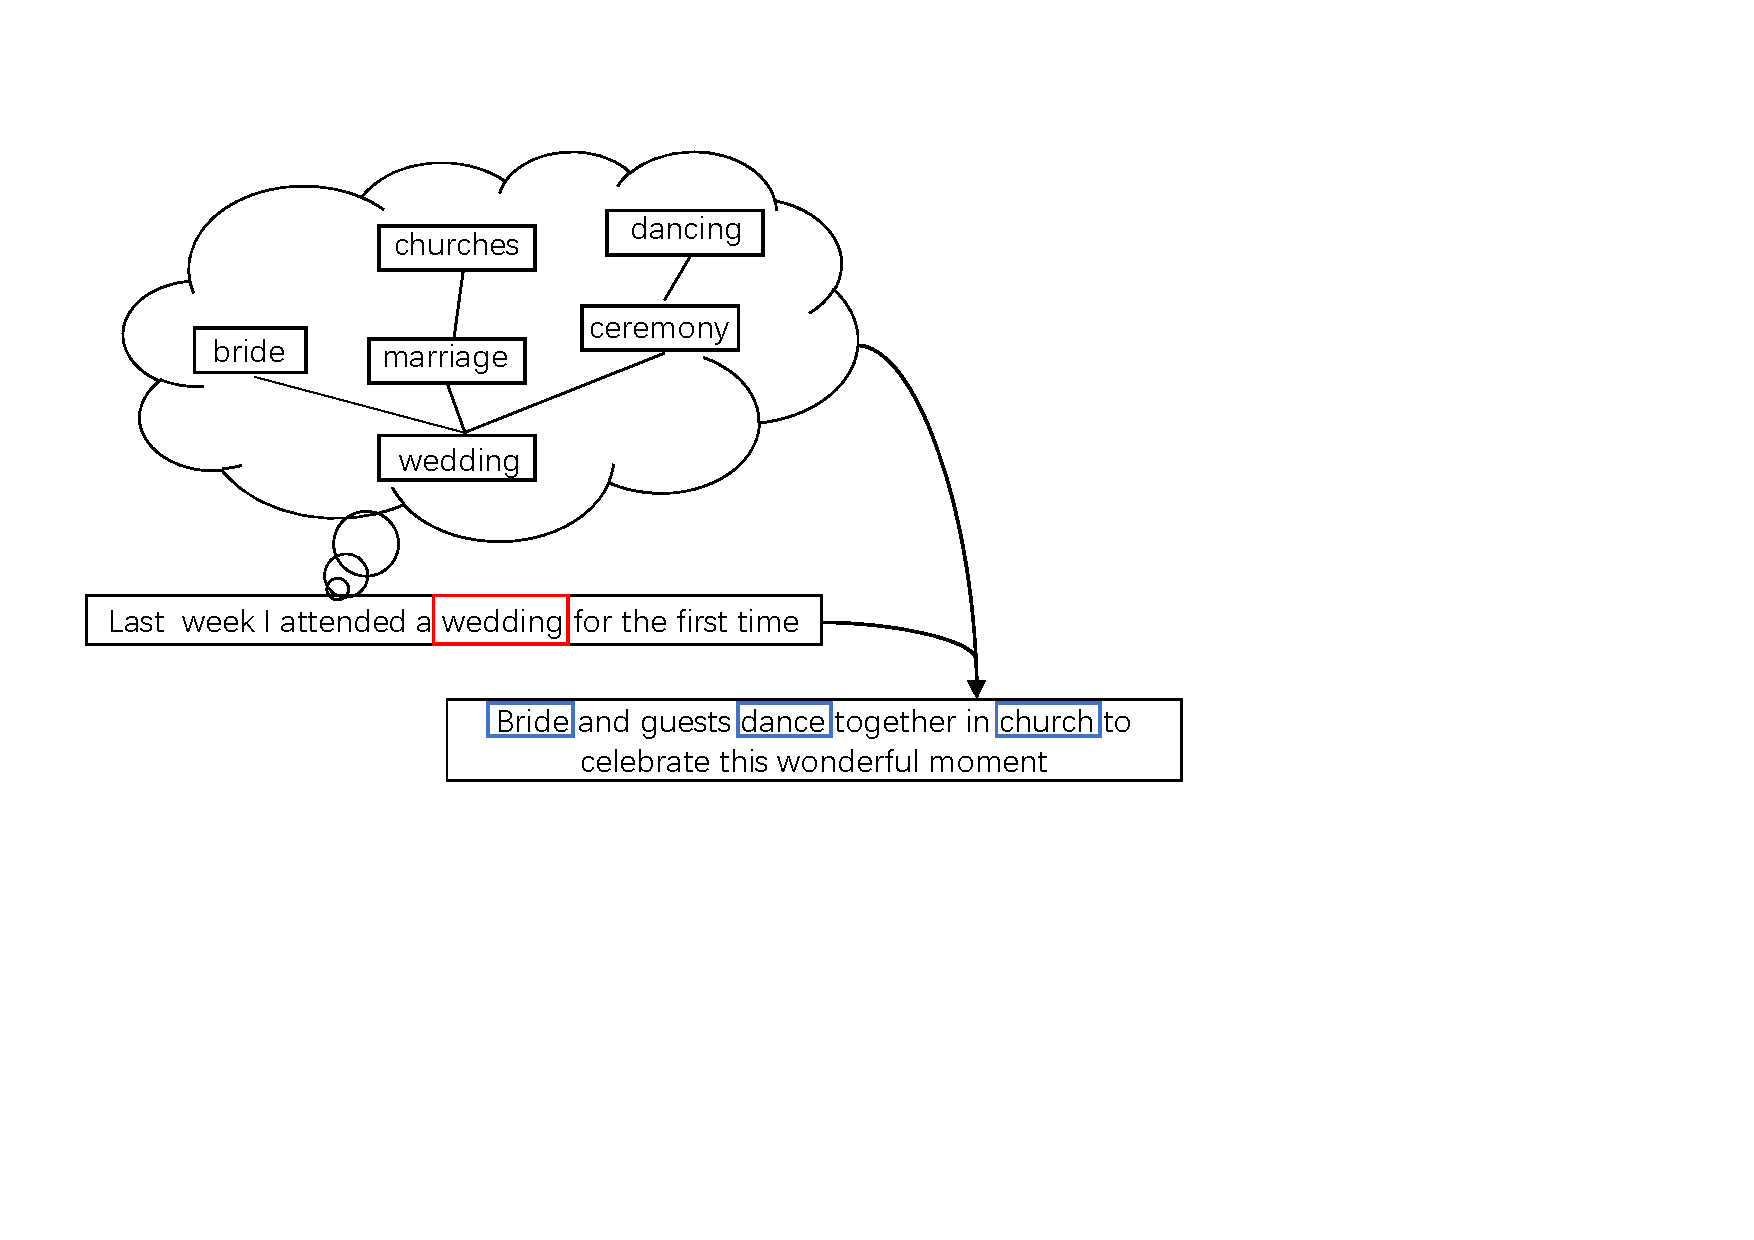
\includegraphics[width=1.0\linewidth]{example.pdf}
% % \includegraphics[\linewidth]{graph_trans.pdf}
% \caption{Illustration of multi-hop reasoning in text generation.   \label{fig:example}}
% \end{figure}

% Modeling semantic connection needs concept path as bridges to connect  two sentences, which needs model enhancing with multi-hop reasoning capacity. For example in the task of story generation, the rest of this story needs to be completed based on such a topic sentence, ``last week i attended a wedding for the first time ''. Human will first imagine some concepts via multi-hop reasoning like that ``wedding $\rightarrow$ bride'',``wedding $\rightarrow$ marriage $\rightarrow$ churches'', 
% % "wedding $\rightarrow$ ring $\rightarrow$ finger", "wedding $\rightarrow$ ceremony $\rightarrow$ bless", 
% ``wedding $\rightarrow$ ceremony  $\rightarrow$ dancing''. Then human can writing coherent based on topic sentence and the those entities with the reasoning path. In this way, human can write informative and interesting long text.

% Most of the current generation models are either a conditional language model or a model with the sequence-to-sequence framework. They have little power to model the conceptual reasoning between sentences as they inherently learn relatively simple patterns of texts and their attention mechanism only extracts and utilizes the internal information. Apparently such model architectures cannot make use of the external knowledge, let alone performing reasoning.
% However it's difficult for current model to do multi-hop reasoning, the reason lies in that  most of current models, either follow traditional encoder-decoder framework, are more likely a black box, 
% do not explicit model entities transferring between sentences, they just generate text word by word, lack of knowledge reasoning, so that it is easier to generate  boring, repetition and irrelevance sentence.  

% To endow text generation models with multi-hop reasoning capacity.

% For example, in the task of story generation, we need to complete the story according to the topic sentence, "last week i attended a wedding for the first time .", human will reason some useful entity and reason path like that "wedding $\rightarrow$ bride", "wedding $\rightarrow$ marriage $\rightarrow$ churches", "wedding $\rightarrow$ ring $\rightarrow$ finger", "wedding $\rightarrow$ ceremony $\rightarrow$ bless", "wedding $\rightarrow$ ceremony  $\rightarrow$ dancing", then condition on current sentence and the reasoned entity with the reason path is used for next sentence writing. With  multi-hop reasoning human can imagine and reason useful  entity, event, and emotion for literary creation, since the human writing text is informative and interesting.  



\begin{figure*}[t]
\centering
\small
\footnotesize
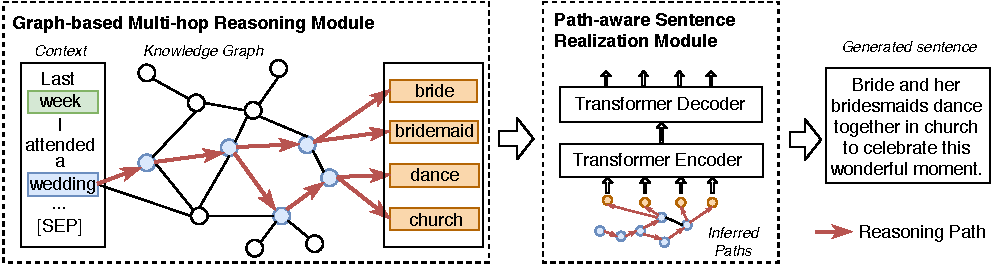
\includegraphics[width=1.0\linewidth]{model.pdf}
% \includegraphics[\linewidth]{graph_trans.pdf}
% \vspace{-0.55in} 
\caption{An illustration about MRG in the inference stage. MRG 
% a sentence-level generative framework by 
iteratively generates a sentence based on previously generated contexts. During each iteration, the reasoning module infers skeleton paths starting from the concepts in the input context. Then this module iteratively searches the neighbor nodes of current path and predicts whether a neighbor node is target concept (ends of the inferred path), intermediate concept (intermediate nodes in the inferred path) or other concept (nodes not in the inferred paths). 
% The module continues searching only for intermediate concepts. 
The sentence realization module is responsible for generating a complete sentence based on the inferred paths. %Then the generated sentence is added to the context to generate the next sentence.
\label{fig:model}}
\end{figure*}

Motivated by human writing, we propose to endow text generation models with the imaginative power. To achieve this goal, we present a novel two-stage approach that imitates the semantic transfer in human writing. In the first stage, a graph-based reasoning module is responsible for inferring paths to select skeleton concepts based on the topic sentence and previously generated sentences via multi-hop reasoning on a knowledge graph. In the second stage, the path-aware sentence realization module approximates the target outputs based on the inferred paths. Owing to the lack of human-annotated training data, we adopt a self-supervised method to generate pseudo parallel corpus to train the two modules.
% Specifically, we treat paths in a knowledge graph from concepts in previously generated contexts to concepts in the target sentence as inferred paths. Then, we take the topic sentence and previously generated sentences as the input, and use the searched paths as the target to train the first module. We also take the searched paths as the input and the next sentence as the target to train the second module.
Experiment results on three long text generation tasks, including story generation,  review generation,  and  product  description  generation show that 
% We conduct experiments on three long text generation tasks, including story generation, review generation, and product description generation. Both automatic and human evaluation demonstrate 
 MRG consistently surpasses existing state-of-the-art generative baselines, such as large-scale pretrained models (e.g., GPT-2) and knowledge-enhanced text generation models, by significant margins, especially in terms of informativeness, diversity and coherence. 
 
 The main contributions are summarized as follows:
% Then, we use the searched paths as input and use the next sentences as the target to train the second module.

%In addition, since not all generation tasks has appropriate knowledge graphs, we also contribute by incorporating an generation-specific knowledge graph construction method to improve the generalization ability of the proposed approach. The key idea is extracting a large graph from a training set via PMI (Point-wise Mutual Information)~\cite{pmi3,pmi2}. PMI is a statistic approach to evaluate the correlation scores between any two words. Higher scores represent two words have tighter semantic dependencies. We regard all words as nodes and use the PMI score to build relations between nodes. Only relations with high PMI scores are kept as relations.  In this way, we can build a large-scale graph based on unstructured training sets. %We conduct experiments on three long text generation task, story generation, review generation, and product description generation. Both automatic and human evaluation demonstrate that MRG consistently surpasses existing state-of-the-art baselines by a significant margin, especially in terms of informativeness and diversity.

% %between two concepts if each of them exists in different sentences and they are connected via $k$ hops in a knowledge graph, and furthermore we train a model that is able to predict the paths .

%Besides,  MRG can improve the quality of the generated text even when there exists no a high-quality artificial knowledge graph, a common situation in many fields and language.


%Specifically, we build a path between two concepts if each of them exists in different sentences and they are connected via $k$ hops in a knowledge graph, and furthermore we train a model that is able to predict the paths . Therefore, in the testing stage the generation system can still perform reasoning with the predictions. This stage is called concept multi-hop reasoning. 


%

% We conduct experiments on three representative task, and both automatic evaluation and human evaluation results show MRG can perform favorable against a series of state-of-the-art baselines.
% modeling conversion of entities, events even emotions between sentences via multi-hop reasoning. To this end,  like some previous work \cite{skeleton_jingjingxu_emnlp8},
% We proposed a two stage method for long text generation. The proposed model has two separate modules, the first module is a graph reasoning module, which is responsible for reasoning and selecting next sentence generation desired entities based on previous generated sentences. The second module is a graph-based sentence realization module, which is responsible for generating readable sentence based on the selected entity with the reason path and previous generated sentences.

% Specifically, our method adopts a sentence-level recurrent generation framework. Before generation a target sentence based on source sentences, i.e., topic sentence and previous generated sentences. It firstly gather nodes  which directly connects with concepts in source sentence in external knowledge graph, such as ConceptNet\cite{concept_net}. Then the graph reasoning module predicts which nodes are useless, which nodes can be  selected as target nodes for target sentence generation and which nodes are intermediate nodes for
% continuing to explore in knowledge graph based on the source sentences. After several above iteration, our method can do reasoning hop by hop, and find useful concepts node with reasoning path for text generation.
% The reasoning process is formulated as a conditional sequence labeling task, and we borrow the power of large pre-trained model Bert \cite{bert} as our multi-hop reasoning module.
% Besides, we can automaticly get training data for multi-hop reasoning with an unsupervised way.
% After several iteration, we can gather desired target nodes and the reasoning path from source sentence to target sentence via some intermediate nodes. Then the sentence realization module  generates target sentence based on source sentences and those target nodes and intermediate nodes. In this way, by modeling concept transferring from source sentence to target sentence, our method can generate long and cohesive text sentence by sentence. We evaluate MRG on two representative long text generation task, story generation and review generation. Both automatic evaluation and human evaluation have shown MRG can perform favorable against a series of strong baselines, especially in term of informative and diversity. Besides, the reasoning path provide a explanatory view for text generation.

\begin{itemize}
\item We propose a novel multi-hop reasoning generation method to learn semantic dependencies among sentences. Unlike previous methods, our proposed model explicitly infers the skeleton path, which provides explanatory views to understand the process of generation. % Our proposed model explicitly learns the semantic dependency by conducting multi-hop reasoning in knowledge graph. 

% \item To the best of our knowledge, this is the first work to study how multi-hop reasoning helps text generation. We view this work as the first step towards learning semantic dependencies via multi-hop reasoning for long text generation.


\item Experimental results show that our approach outperforms state-of-the-art baselines especially in terms of informativeness, diversity and coherence.
% Our analyses demonstrate the efficiency of our method in long range semantic dependencies modeling.



% our works point a new direction for long text generation, i.e., imitating human writing process to model semantic connection among sentence  via multi-hop reasoning in knowledge graph.
% \item We build Self-constructed Graph for each task, so that MRG can perform complex reasoning even there exists no a ready-made knowledge graph.


\end{itemize}

% Our methods can be expended to arbitrary long text generation task, even for those tasks which have not a good concept overlap with inter-graph ConceptNet. We built a Self-constructed Graph for those tasks according point-mutual-information, which also show large improvement in text quality in term of informative and diversity. We conduct various experiments in three different dataset, story generation, comment generation, and summary generation,

% Reasons lie in that it's difficult for a traditional Seq2Seq model captures the entity and event relation between current sentence and next sentence. 

% \begin{figure}[t]
% \centering
% \footnotesize
% 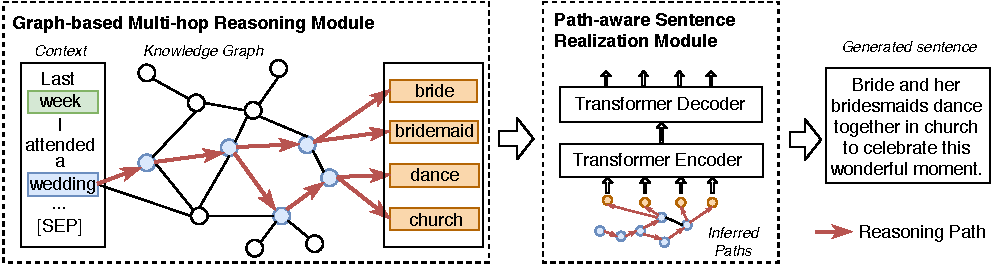
\includegraphics[width=1.0\linewidth]{model.pdf}
% % \includegraphics[\linewidth]{graph_trans.pdf}
% \caption{Illustration of  MRG\label{fig:example}}
% \end{figure}



% \section{Preliminaries}
% \label{sec:preliminary}
% In this section, we introduce necessary notations and formalize the task of long text generation. Suppose we have a parallel long text generation data set 
% $\mathcal{P}$. Each parallel sample consists of a source context $x$, and a corresponding target output $\bm{y}$ containing $n$ sentences $\{y_1, y_2,\dots, y_n\}$. Formally, long text generation requires the generation system to generate a 
% % grammatical, semantically coherent and pragmatically cohesive 
% informative and coherent
% long text $\bm{y}$ based on the source input $x$. The training objective for the model is that the generation should approximate the target $y$. 

% However, unlike machine translation that generates aligned information to the source context, long text generation requires the system to generate more novel contents. It is common that the source information is not sufficient enough for the generation of a long text. A solution that has proved effective is to generate the text sentence by sentence. To be more specific, when generating the $j$-th sentence $y_j$, the generation system takes both the source context $x$ and the previous generation $\bm{y_{<j}}$ as the input. 
 
% This solution can alleviate the problem of long-term dependency. Still, the generation system suffers from the problem of insufficient input and the lack of knowledge and reasoning ability so that it is hard for it to generate a long text with much new information that does not exist in the source context. Therefore, we make use of knowledge graph for reasoning. We denote the given knowledge graph as $\mathcal{G}$ and its $m$ entities as $\{v_1,v_2,\cdots,v_m\}$. %If there is a path between two entities $v_1$ and $v_2$, the entities are believed are connected. The $k$ entities in the path are called intermediate entities, and $v_1$ can reach $v_2$ via $k+1$ hops.

\section{Proposal}
In this section, we introduce our proposed two-stage approach, \textbf{M}ulti-hop \textbf{R}easoning \textbf{G}eneration (\textbf{MRG}). We first give the formulation of long text generation and the related notations. Then, we provide an overview of our approach and introduce the two modules.

\subsection{Formulation and Notations}
% \medskip\noindent\textbf{Problem Formulation}\hspace{1em} 
% Suppose we have a parallel long text generation dataset 
% $\mathcal{P}$. 
Given a parallel long text generation dataset, each parallel sample consists of a source context $x$, and a corresponding target $\bm{y}$ containing $n$ sentences $\{y_1, y_2,\dots, y_n\}$. Formally, long text generation requires the generation system to generate an 
% grammatical, semantically coherent and pragmatically cohesive 
informative and coherent
long text $\bm{y}$ based on the source input $x$. %The training objective for the model is that the generation should approximate the target $y$. 
 
MRG adopts a sentence-level generative framework to learn semantic dependencies among sentences, which takes both the source context $x$ and the previous generation $\bm{y_{<j}}$ as the input when generating the $j$-th sentence $y_j$. Besides, a knowledge graph $\mathcal{G}$ is needed for MRG to conduct semantic transfer via multi-hop reasoning, and $\bm{v}=\{v_1,\dots,v_m\}$ is the set of  $m$ nodes on $\mathcal{G}$.


\subsection{Overview}
The architecture illustration of the proposed MRG model is shown in Figure~\ref{fig:model}. 
% MRG consists of two modules: the graph-based multi-hop reasoning module and path-aware sentence realization module. 
% We adopt a sentence-level text generation framework where the complete text is generated sentence by sentence.  
% MRG generate the complete text sentence by sentece.
%takes the previously generated context as input and
At each sentence-level generation,
the reasoning module first infers skeleton paths from a knowledge graph to imitate the imagination in the human writing for coherent sentence-level semantic transfer. 
Specifically, the inferred paths start from the concepts in the input sentences for initialization. The reasoning module iteratively adds new nodes into the inferred paths. At each reasoning step, the module first finds all neighbor nodes of current inferred paths as candidate nodes and predicts their labels. We define three kinds of labels, including \textbf{target concept} (ending of the inferred path), \textbf{intermediate concept} (middle node in the inferred path), and \textbf{other concept} (node not in the inferred path). For intermediate concepts, the module adds them into the inferred path and keeps the reasoning process. 
For target concepts, the module adds them to the inferred path and stops the reasoning process. For other concepts, the module just stops the reasoning process. We treat the inferred skeleton paths as pivots connecting semantics among sentences. Then, the realization module takes the inferred paths as inputs and decodes a complete  sentence. %The details of two modules and training algorithms are shown in the following.  


%Generally, the reasoning module searches the concepts on the given knowledge graph, with multiple hops from those in the source input, and finds out the target concepts and intermediate concepts, which contribute much to the generation. 
%In the training stage, target concepts refer to the concepts in the subsequent target context. The concepts on the multi-hop search path to the target concepts are intermediate concepts. The other concepts are named as unrelated concepts. 
%The reasoning module learns to predict whether a neighbor of a concept in the source input is a target concept, intermediate concept or unrelated concepts. 
%In the inference stage, the reasoning module searches the neighbors of the concepts in the input and predict their types. If a neighbor is a target concept or an unrelated concept, the search on that path ends, but if it is an intermediate concept, the search continues and the module repeats the prediction process. 
%Therefore, this module can provide target concepts and intermediate concepts to the next module without the target context. 
%Then the sentence realization module, a Transformer-based model,  generates a sentence with the extracted concepts from the reasoning module, instead of solely the source input. 
%In the following, we introduce the details of our approach and focus on the two key modules.


% The first module is a conditional sequence labeling model, since it's vital to selected correct nodes as targets node to generate next sentence, we adopts the powerful pre-trained model, which has shown their great power in many fields,  as the reasoning module, to predict a  triple sequence of whether each node is selected as target nodes or as intermediate nodes, nor discarded as useless nodes. The second module is a sequence-to-sequence model to organize the target words and intermediate nodes selected by first module as input  to generate a target sentence. Moreover, To reduce the risk of error propagation between the two module, we introduce a denoising data augmentation methods for the second module.
% \subsection{Preprocessing: prepare training data }
% \subsection{Preliminaries}

\subsection{Graph-based Multi-hop Reasoning}
The graph-based multi-hop reasoning module is responsible for learning the semantic dependencies among sentences via conceptual paths. 
This module explores on the knowledge graph to find a path that can connect concepts in the context with concepts in its subsequent sentence through intermediate concepts. 
Specifically, for a concept $v_1$ in a source sentence and $v_2$ in its subsequent sentence, their connected path is essential to semantic transfer.
% In our multi-hop reasoning method, we first extract concepts from both the source and target context.
% , which are labeled as \textbf{source concepts} and \textbf{target concepts}. 
% Specifically, for sentence-by-sentence long text generation, the source context is the previous generation, and the target of the next sentence to generate. 
MRG performs reasoning on a knowledge graph, which starts at the concepts in the source sentence and ends at the target concepts. The inferred concept chains form multiple conceptual reasoning paths.
% The concepts on the paths are labeled as \textbf{intermediate concepts}, and the others are labeled as \textbf{other concepts}. 
% With the training data and the labeled concepts, the reasoning module performs conditional sequence labeling. 
In the implementation, the reasoning module performs sequence labeling for nodes in a knowledge graph conditional on source input.
Concretely, at the $1$st hop, the input for the module is a sequence of the source context and their concepts on the graph $\bm{T^{(1)}}=\{x_1, \dots,x_{n},\mathtt{[SEP]},v^{(1)}_1,\dots,v^{(1)}_m\}$. The reasoning module learns to predict their labels of the concepts. 
When reaching an intermediate concept, MRG moves to the next hop and collects its neighbors.
% and adds the intermediate concepts and target concepts to the source context. 
The reasoning of neighbors continues and the module repeats the learning of sequence labeling until it meets concepts other than intermediate ones or the module reaches the max number of hop.
% already performed $k$ hops.  
In the inference stage, the reasoning module infers multiple paths and finds out possible target concepts and intermediate concepts. 
% More specifically, starting from any source concept, the module searches its neighbors and predict their labels. Unless it predicts an intermediate concept, the search at that path ends. For a prediction of intermediate concept, the search continues and repeats the aforementioned process. 
We adopt the powerful pretrained model BERT~\cite{devlin-et-al:bert} as the backbone. Below we provide more details of the module. 

% Specifically, for a sentence $x=\{x_1,x_2,\dots,x_n\}$, we extract the words that are also entities in the knowledge graph and form an entity sequence $v^0=\{v^0_1, v^0_2, \dots,v^0_m\}$. Then we choose the entities labeled with $2$ in $v^0$, collect their neighbor entities and form another entity sequence $v^1$, the entity sequence for the first hop. Similarly, for the $i^{th}$ hop, $v_i$ is a sequence of the neighbor entities of the ones labeled with $2$ in $v^{i-1}$. Finally, we concatenate $x$ and $v^i$ with a token ``[SEP]'' and form a new sequence $T^i=\{x,[SEP],v^i\}=\{x_1, x_2,\dots,x_n,[SEP],v^i_1,v^i_2,\dots,v^i_m\}$, which represents the input of the $i^{th}$ hop. In the following, we introduce the architecture of the module, including the BERT encoder and the classifier.

% given a source sentence $x=\{x_0,x_1,\dots,x_n\}$.  At the first reasoning hop, we collect all the word which appear in source sentence and also is a node in knowledge graph,  the collected search words set is denoted as  $\{v^1_0, v^1_1, \dots,v^1_m\}$, then we concatenate source sentence and search words set,  we use a special token ``[SEP]'' separation the two parts, which is recommended by the original paper. We set label of words in  source sentence as default CrossEntropy ignore index, in this way the source sentence parts is not calculated loss when training, they just act as a conditional part to supply needed information for reasoning. For the other reason level. At the i'th reasoning hop, we collected the neighbor words of last reasoning hop the module given label 2, then search words set can be denoted as $V_i = \{v^i_0, v^i_1, \dots,v^i_m\}$. The word sequence which is emit to multi-hop Reasoning Module at i'th reasoning hop can be denoted as
% $T_i=\{x,[SEP],V_i\}=\{w_0, w_1,\dots,w_n,[SEP],v^i_0,v^i_1,\dots,v^i_m\}$.
% At the $k$-th hop, the input for the reasoning module is $\bm{T^{(k)}}=\{x_1, \dots,x_{n},\mathtt{[SEP]},v^{(k)}_1,\dots,v^{(k)}_{l}\}$, where $l$ is the number of neighbors of the previous intermediate nodes.
% \subsubsection{Bert encoder}
\medskip\noindent\textbf{BERT-based Labeller}\hspace{1em}
The module is a sequence labeling model with BERT as the encoder. 
The goal of BERT encoder is to provide a representation for conditional sequence labeling. At the $k$-hop reasoning step, it takes $\bm{T^{(k)}}=\{x_1, \dots,x_{n},\mathtt{[SEP]},v^{(k)}_1,\dots,v^{(k)}_{l}\}$ as the input, where $l$ is the number of neighbors of the previous intermediate nodes, and generates hidden representations:
\begin{equation}
\bm{h^{(i)}}= BERT(\bm{T^{(i)}}),
\end{equation}
where $\bm{h^{(i)}}$ is a vector sequence. Each vector is the representation of the word at the corresponding position. 
For  simplicity, we omit the details of BERT, and refer the readers to the original work~\cite{devlin-et-al:bert}.

% \medskip\noindent\textbf{Labeller.}\hspace{1em}
On top of the BERT encoder, we add a classifier layer for labeling based on Multi-Layer Perceptron (MLP). The input of the classifier is the  representation in the last layer of the BERT encoder $\bm{h^{(i)}}$. The following computation demonstrates how to predict the label $l_r$ at position $r$:
% The output representation of each position is then sent to a classifier to predict label of each words. Comply with the recommendations in the original Bert paper, we adopt a simple MLP to compute the probability distribution of the label $p_i(l_i|T_i)$:
\begin{equation}
p(l_r|\bm{h^{(i_r)}}) = softmax(\bm{W_c}\bm{h^{(i_r)}}+b_c),
\end{equation}
where $\bm{W_c}$ and $b_c$ are the weight matrix and bias term. We mask  the losses of  context words when doing sequence labeling.

% \medskip\noindent\textbf{Data Collection for Module Two}\hspace{1em}
% After the process of multi-hop reasoning, the target concepts are added to the target concept set $W^T_{set}$, and intermediate concepts are added to the intermediate concept set $W^I_{set}$. The two sets of words are significant inputs for the module, which is illustrated in the following.
% \subsubsection{Construct Supervisory Signals}


\subsection{Path-aware Sentence Realization}
The path-aware sentence realization module aims at generating a sentence that approximates the target based on the inferred paths. 
% the module for sentence realization is based on the sequence-to-sequence framework, 
We adopt the architecture of Transformer~\cite{vaswani-et-al:transformer} for sentence realization.
% due to its supreme performances in a series of generation tasks. 
In the following, we illustrate the details of data preparation and module architecture. 
% This module follows the traditional sequence-to-sequence framework, and we adopt Transformer  as the sentence realization module. 

\medskip\noindent\textbf{Data Preparation}\hspace{1em}As shown in Figure~\ref{fig:model}, we extract the inferred paths from the knowledge graph $G$ to build a sub-graph $G'_{x,y<t}$ for sentence realization. Specifically, for each concept $\hat{n}^{(i)}$ in inferred target concepts set $\bm{\hat{n}}$, without changing the topology of the nodes that directly connect to $\hat{n}^{(i)}$ on $G$, we also connect the intermediate nodes in the reasoning path which can point to $\hat{n}^{(i)}$ with $\hat{n}^{(i)}$. In this sub-graph all the intermediate concepts directly connect with its corresponding target concepts.
% As shown in Figure \ref{fig:model}, we build a sub-graph $G'_{x,y<t}$ as 
% the input for sentence realization based on the concepts in source text $x$ and  the previous target text $\bm{y_{<t}}$ (it refers to the previous generation during the inference stage), the target word sets $W^T_{set}$ and intermediate words set $W^I_{set}$ and the given knowledge Graph $G$. Specifically, We take concepts in $W^T_{set}$ as main concepts, denoting as $\hat{n}$. For each concept $\hat{n}^i$ in $\hat{n}$, we connect the concepts in the inferred path which point to $\hat{n}^i$ and the concepts in $W^I_{set}$, $x$ and $\bm{y_{<t}}$ which  directly connect with the $\hat{n}^i$ in $G$ with $\hat{n}^i$ to build the sub-graph $G'_{x,y<t}$.

% firstly we connect the concepts in the inferred path which point to $\hat{n}^i$ and the concepts in $W^I_{set}$, $x$ and $\bm{y_{<t}}$ which  directly connect with the $\hat{n}^i$ in $G$ with $\hat{n}^i$ to build the sub-graph $G'_{x,y<t}$.

\medskip\noindent\textbf{Transformer}\hspace{1em} It builds upon on a encoder-decoder framework.
% As it is limited in generating long texts, we use Transformer to generate the text sentence by sentence. 
For each node in target node set $\bm{\hat{n}}$ of the input graph $G'_{x,y<t}$, we concatenate its directly linked nodes as its features. Then we use the sum of target node embedding and its feature node embeddings as node representation. The node representation of $\bm{\hat{n}}$ is denoted as $\bm{\hat{e}}$. On the transformer encoder, we find modeling the order of paths is more complicated but cannot improve the final results, so we remove the positional encoding to eliminate the effects of reasoning order.
The Transformer encoder (TrmEnc) encodes $\bm{\hat{e}}$ to a list of representations $\bm{\hat{h}}$: 
% For the target words in $G^{`}$, we add all connected intermediate words embedding to corresponding target word embedding which can be denoted as $V^o=\{v^o_0, v^o_1,\dots, v^o_m\}$. Then we use a special token ``[SEP]'' to separate  source sentence and target words. The input can be formulated as $q=\{x,\bm{y_{<t}},[SEP],V^o\}$
\begin{equation}
\bm{\hat{h}} = TrmEnc(\bm{\hat{e}}). \\
\end{equation}
At the $i-{th}$ decoding time step, the Transformer decoder (TrmDec)  generates a probability distribution for word prediction by attending to both $\bm{\hat{h}}$ and previous decoder outputs:
\begin{equation}
\begin{split}
p(y_{i,t}|\bm{y_{<i,t}}, \bm{\hat{h}}) &= TrmDec(\bm{y_{<i,t}}, \bm{\hat{h}}). \\
% p(y_t|y_{<t}, h^j) &= softmax(W_pv_t + b_p)
\end{split}
\end{equation}
Both the encoder and decoder consist of multiple layers, each with a multi-head self-attention sub-layer and a point-wise feed-forward neural network (FFN) sub-layer, and each of the layers of the decoder has an additional encoder-decoder attention sub-layer.
% \subsection{Training and Inference}
% In the training stage, 
% % the objective functions of 
% the two modules are optimized using cross entropy loss.
% In the inference stage, the two modules work together following a two-stage framework. In the first stage, the reasoning module infers several conceptual paths and emits the paths with the realization module . In the second stage,  the realization module decodes a sentence based on the inferred paths.


\medskip\noindent\textbf{Pseudo Parallel Data Construction}\hspace{1em}Owing to the lack of human-annotated training corpus, we adopt a self-supervised approach to construct peseudo parallel data to train our two modules. 
% We extract data from the training set and build a dataset. 
% Specifically, similar to the data for next sentence prediction in Devlin et al.~\citet{devlin-et-al:bert}, we extract sentence pairs from a text with multiple sentences.
% Specifically, we treat paths in a knowledge graph from concepts in previously generated contexts to concepts in the target sentence as inferred paths. Then, we take the topic sentence and previously generated sentences as the input, and use the searched paths as the target to train the first module. We also take the searched paths as the input and the next sentence as the target to train the second module.
% We extract sentence pairs from a text with multiple sentences in training data. 
% In fact, the former one in the pair can be a longer paragraph with multiple sentences, and the latter one is the subsequent sentence. 
% For training the first reasoning modules, we define the co-occurence entity when starting from the source sentence go through several intermediate nodes in knowledge graph that can meet entity in target sentence, then we call the nodes in target sentence as target nodes, and the other nodes in this path as intermediate nodes. 
% Algorithm 1 illustrates the process of automatically annotating the reasoning sequence. 
% Given a long text, We first cut the long text into the form of sentence pairs, of each pair consist of directly connected sentences, we call them  source sentence and target sentence.
Given a long text, we first cut the long text into the form of sentence pairs, of each pair consist of two consecutive sentences.
For each sentence pair, we search the concepts that exist in the knowledge graph. If a concept $v_1$ in the former sentence can reach a concept $v_2$ in the latter sentence via $k+1$ hops, the path with $k+1$ nodes are labeled. To be specific, $v_2$ is labeled as target concepts, $v_1$ and $k$ intermediate nodes are labeled as intermediate concepts. We set a constraint for the  max number of hops and neighbors of a concept to avoid over-exploration. Then, we collect  pairs with at least one labeled path to form a dataset for sequence labeling. Besides, we collect the pairs of paths with its subsequent sentence to form a dataset for sentence realization.
% conditional sequence labeling. 
% Training a reasoning module with a conditional sequence labeling task can provide the reasoning module with the ability to find out the paths in the knowledge graph that benefits generation. 
% In the following, we introduce both the module architecture and the training details.


% \subsection{Multi-hop Reasoning}
% The first stage of our approach is the multi-hop reasoning on knowledge graph. In this stage, the system performs reasoning on a given knowledge graph and extracts key information that can benefit the generation. Specifically, for an entity $v_1$ in a sentence and $v_2$ in its subsequent sentence, if there is a path between the two entities on the knowledge graph $\mathcal{G}$, we believe that the path is essential to the reasoning. Therefore, we extract a dataset from the training data of text generation and build a model for reasoning. The model learns to predict the paths without the information of the subsequent context. In the following, we first introduce the data preprocessing and the details of the module.


% \subsubsection{Preprocessing}
% A module of reasoning in a system of long text generation should be able to predict the relevant entities in its subsequent generation $\bm{y_{>t}}$ based on the entities source context $x$ and its previous generation $\bm{y_{<t}}$.
% For training such a reasoning module, we extract data from the training set and build a novel dataset. Specifically, similar to the data for next sentence prediction in \citet{bert}, we extract sentence pairs from a text with multiple sentences. In fact, the former one in the pair can be a longer paragraph with multiple sentences, as if the latter one is the subsequent sentence. 
% % For training the first reasoning modules, we define the co-occurence entity when starting from the source sentence go through several intermediate nodes in knowledge graph that can meet entity in target sentence, then we call the nodes in target sentence as target nodes, and the other nodes in this path as intermediate nodes. 
% % Algorithm 1 illustrates the process of automatically annotating the reasoning sequence. 
% % Given a long text, We first cut the long text into the form of sentence pairs, of each pair consist of directly connected sentences, we call them  source sentence and target sentence. 
% For each sentence pair, we find out the words that exist in the knowledge graph. If an entity $v_1$ in the former sentence can reach an entity $v_2$ in the latter sentence via $k+1$ hops, the path with $k$ intermediate nodes are labeled. To be specific, $v_2$ labeled with $1$, $v_1$ and the intermediate entities are labeled with $2$, and the other entities in the pair are labeled with $0$. We set $k$ to 1 and set a constraint for the number of neighbors of an entity in case of over-exploration. Then, we collect the pairs with at least one labeled path, extract the labeled entity sequences and thus form a dataset for sequence labeling. 
% Training a reasoning module with a sequence labeling task can provide the reasoning module with the ability to find out the paths in the knowledge graph that benefits generation. In the following, we introduce both the module architecture and the training details.
% % Then for each word in source sentence if this word also appear in knowledge graph, then we enumerate  all of  it's the multi-hop path (we also can constrain the width of search for the node which has too many neighbour nodes in knowledge graph, In this situation, we can random choice a subset of it neighbour nodes). In order not to explore too many paths, we limit the maximum number of hops to two. Then if a end nodes in search path also appear in target sentence, we call the nodes as target nodes and the node label is  set to 1, other nodes in this path set as intermediate nodes, labelling with 2. Then for other nodes that does not appear in target sentence and can not reach target via hopping in knowledge graph, we label them with 0. 
% % we collect all sentence pair that at least one multi-hop reasoning path is exists from source sentence to  target sentence. We random drop some node with label of 0, avoiding the label sequence is too long. In this way, we can obtain a triple sequence with the 0/1/2 label denoting whether this node in knowledge graph is used for next sentence generation, or as a intermediate node for continuing search or just a useless nodes. The  triple sequence will be regard as the supervised signal for training the multi-hop reasoning module. And the selected target nodes with intermediate nodes as feature and source sentence are used to emit the the target sentence.

% \subsubsection{Graph-based Multi-hop Reasoning Module}
% As mentioned above, we formulate the multi-hop reasoning as a conditional sequence labeling task and build a corresponding dataset for training the module. We adopt the powerful pre-trained model Bert \cite{bert} as the backbone of the multi-hop reasoning module due to its outstanding performance in a series of downstream tasks. 
% % 一个问题是为什么要这么设计输入,理由是什么,我这里先解释为第一部分输入全句是因为可以观察到上下文 
% % 是的，为了观察到上文
% Specifically, for a sentence $x=\{x_1,x_2,\dots,x_n\}$, we extract the words that are also entities in the knowledge graph and form an entity sequence $v^0=\{v^0_1, v^0_2, \dots,v^0_m\}$. Then we choose the entities labeled with $2$ in $v^0$, collect their neighbor entities and form another entity sequence $v^1$, the entity sequence for the first hop. Similarly, for the $i^{th}$ hop, $v_i$ is a sequence of the neighbor entities of the ones labeled with $2$ in $v^{i-1}$. Finally, we concatenate $x$ and $v^i$ with a token ``[SEP]'' and form a new sequence $T^i=\{x,[SEP],v^i\}=\{x_1, x_2,\dots,x_n,[SEP],v^i_1,v^i_2,\dots,v^i_m\}$, which represents the input of the $i^{th}$ reasoning hop. In the following, we introduce the architecture of the module, including the BERT encoder and the classifier.

% % given a source sentence $x=\{x_0,x_1,\dots,x_n\}$.  At the first reasoning hop, we collect all the word which appear in source sentence and also is a node in knowledge graph,  the collected search words set is denoted as  $\{v^1_0, v^1_1, \dots,v^1_m\}$, then we concatenate source sentence and search words set,  we use a special token ``[SEP]'' separation the two parts, which is recommended by the original paper. We set label of words in  source sentence as default CrossEntropy ignore index, in this way the source sentence parts is not calculated loss when training, they just act as a conditional part to supply needed information for reasoning. For the other reason level. At the i'th reasoning hop, we collected the neighbor words of last reasoning hop the module given label 2, then search words set can be denoted as $V_i = \{v^i_0, v^i_1, \dots,v^i_m\}$. The word sequence which is emit to multi-hop Reasoning Module at i'th reasoning hop can be denoted as
% % $T_i=\{x,[SEP],V_i\}=\{w_0, w_1,\dots,w_n,[SEP],v^i_0,v^i_1,\dots,v^i_m\}$.

% % \subsubsection{Bert encoder}
% \medskip\noindent\textbf{Bert Encoder}\hspace{1em}
% The goal of BERT encoder is to provide a representation for conditional sequence labeling. More specifically, the encoder encodes the input sequence $t^i$ and generates a new representation $h^i$:
% \begin{equation}
% h^i= BERT(T^i)
% \end{equation}
% where $h^i$ is a vector sequence where each vector is the representation of the word at the corresponding position. 
% For the purpose of simplicity, we omit the details of BERT, and refer the readers to the original work \cite{bert}.

% \medskip\noindent\textbf{Classifier}\hspace{1em}
% On top of the BERT encoder, we add a classifier based on Multi-Layer Perceptron (MLP). The input of the classifier is the output representation of the BERT encoder $h^i$. The following computation demonstrates how to predict the label $y_t$ at position $t$:
% % The output representation of each position is then sent to a classifier to predict label of each words. Comply with the recommendations in the original Bert paper, we adopt a simple MLP to compute the probability distribution of the label $p_i(l_i|T_i)$:
% \begin{equation}
% p(y_t|h^i_t) = softmax(W_ch^i_t+b_c)
% \end{equation}
% Where $W_c$ and $b_c$ are the weight matrix and bias term. 

% % \medskip\noindent\textbf{Data Collection for Module Two}\hspace{1em}
% After the process of multi-hop reasoning, the words labeled with $1$ are added to the target word set $W^T_{set}$, and those labeled with $2$ are added to the intermediate word set $W^I_{set}$. The two sets of words are significant inputs for the Path-aware sentence realization Module, which is illustrated in the following.
% % After each reasoning hop, for each word labeled as 1, then  we add those words to target words set $W^T_{set}$. For each word labeled as 2, then we add those words to intermediate words set $W^I_{set}$.


\subsection{Self-constructed Graph for MRG}
Although there are several widely-used artificial knowledge graphs, such as ConceptNet~\cite{liu-singh:concept_net}. However, for some specific fields, 
% we are still lacking in high-quality knowledge graphs. 
we still lack in an artificial knowledge graph. 
To make MRG applicable in such scenarios,  we propose to build a graph based on the training data. Inspired by~\citet{textgcnPMI,pmigraph}, we build a graph via PMI (Point-wise Mutual Information)~\cite{andrew-et-al:pmi3}, a popular measure for word associations. The behind motivation is that words in the same text are more likely semantically connected, so we can connect those words with edges to build a graph called as Self-constructed Graph. Specifically, we compute the PMI between any two words in the training vocabulary except for stop words with:
% To tackle the problem, we propose a method to build a knowledge graph based on the training data. Specifically, we build a knowledge graph via PMI (Point-wise Mutual Information)~\cite{andrew-et-al:pmi3,su-et-al:pmi2}. The behind motivation is that words in the same text more likely share the same topic, so we can connect those words with the same topic with edges and build a knowledge graph, which is called as Self-constructed Graph. Specifically, we compute the PMI between any two words in a vocabulary except for stop words with:
\begin{equation}
\begin{split}
PMI(w_i;w_j) = log\frac{p(w_i,w_j)}{p(w_i)p(w_j)} 
% p(y_t|y_{<t}, h^j) &= softmax(W_pv_t + b_p)
\end{split}
\end{equation}
where $p(w_i, w_j)$ refers to the probability of the two words $w_i$ and $w_j$ in the same text. $p(w_i)$ and $p(w_j)$ are the probabilities of words in the entire training data. For each words, we connect those words with top-$k$ PMI values.

% We highly recommend reader to read the original paper \cite{Transformer} for the detailed architecture information of Transformer.

% \subsection{Inference}
% At the inference stage, 

% we firstly use Graph multi-hop reasoning module to reason some desired target nodes and intermediate nodes based on 
% source sentence x and previous generated sentence $y_{<t}$. Specifically, we get the label of each nodes by:

% \begin{equation}
% \hat{l}^i_t = \mathop{\arg\max}_{l^i_t \in \{1,2,3\} } p_i(l^i_t|Q)
% \end{equation}
% The word with $\hat{l}^i_t=1$ is added to target word set $\kappa_t$ the word with $\hat{l}^i_t=2$ is added to intermediate word set $\kappa_i$, while that with  $\hat{l}^i_t=0$ is discared. 

% Then sentence realization module take those as input to generate t'th target sentence:
% \begin{equation}
% \hat{y}^i_t = \mathop{\arg\max}_{y^i_t \in \mathcal{V} } p_w(y_t|\bar{Q})
% \end{equation}
% Where $\mathcal{V}$ is the decoder vocabulary of the model. This decoding process keeps running until it generates an ending token or the maximum sequence length is reached. 

% \subsection{sentence realization Denoising}
% Our proposed method can be categorize into two-stage method 
% \cite{}, since error may propagate when the first module somehow cannot reason desired target nodes. To remedy this, inspired by \citet{unsupervised_nmt}, we add a denoising task for the sentence realization module to reduce the hurt from error propagation and improve the robustness of our model. Specifically, when preparing training data for module two, we random drop target words and add insert some words does not label as target words. The target words dropout simulates the case when the reasoning module can not reason the desired target words, The random words inserting simulates the case when the reasoning module misread a other nodes as target nods. Those noising data, acting as adversarial examples, is able to improve the robustness of module two when generating target sentence.

\section{Experiments}
% We evaluate our method on three long text generation tasks, including story generation, review generation and product description generation.
% In the following, we introduce the details of our experiments.

\subsection{Dataset}
Here we describe the used datasets and  Table~\ref{tab:dataset} demonstrates the detailed statistics.

\medskip\noindent\textbf{Story Generation}\hspace{1em}This dataset comes from a visual storytelling dataset~\cite{huang-et-al:visualstory} which consists of pairs of an image sequence and a human-written story. 
Following ~\citet{xu-et-al:skeleton_jingjingxu_emnlp8}, we only use the text data for our experiments.
For each story, we extract the first topic sentence as the source input and the rest of the story as the target. 

\medskip\noindent\textbf{Review Generation}\hspace{1em}This dataset is provided by Yelp
Challlenge\footnote{https://www.yelp.com/dataset/challenge}.
% contains user reviews on Yelp.
Similarly, for each review, the first sentence is the source input and the rest is the target.

\medskip\noindent\textbf{Description Generation}\hspace{1em}This dataset is crawled from Taobao\footnote{www.taobao.com}, 
a Chinese e-commerce platform. It consists of pairs of product titles and the corresponding product descriptions, which are composed by professional content producers on the website. We discarded pairs with a description less than 20 tokens or longer than 150 tokens to remove noisy samples. We will release this dataset if this paper is publised.%~\footnote{.}

% The dataset statistics are shown in Table 3. For story generation, we use the standard split. For review generation and description generation, we randomly sample 5K, 5K as test and development set, the rest is  training set.

% \subsection{Evaluation Metrics}
% We evaluate the diversity and novel of each generated text by automatic evaluation. 
\subsection{Baselines}
% Here we implement several widely-used long text generation methods, and some pre-trained model as our baseline models. The details
% We compare our models with three types of baseline models: widely-used text generation models (Seq2Seq, Transformer), two stage skeleton-based method (SkeletonSeq) and the large scale pre-trained model (GPT2). 
We compare our models with the following widely-used text generation approaches.
\begin{itemize}
\item \textbf{Seq2Seq}~\cite{sutskever-et-al:seq2seq} with attention mechanism~\cite{bahdanau-et-al:attention} is a widely-used model for text generation.
\item \textbf{Transformer}~\cite{vaswani-et-al:transformer} is the state-of-the-art architecture for 
a series of tasks of nature language generation. 
% \item \textbf{Seq2Seq-K} is similar to Seq2Seq model, we concatenate knowledge entity that directly connected in knowledge graph with word in source sentence, we also enhance copy mechanism to this model called \textbf{Seq2Seq-KC}. 
% \item \textbf{Transformer-C} is similar to Transformer. We concatenate the source input with the concepts directly connected to words of the source in the knowledge graph. Furthermore, we apply Copy mechanism \cite{copy} to enhance the capabilities of the model. Specifically, \textbf{Transformer-CC} denotes the model trained with the concepts in ConceptNet, and  \textbf{Transformer-CI} denotes the model trained with the concepts in Self-constructed Graph.
% \item \textbf{GPT} is a large pre-trained model 
\item \textbf{Skeleton2Seq}~\cite{xu-et-al:skeleton_jingjingxu_emnlp8} is a two-stage generative method, which first generates a skeleton and then expands it to a complete sentence. This method also uses the sentence-level recurrent generation framework.
\item \textbf{Plan\&Write}~\cite{plan-and-write} is a two-stage generative method, which first generates a sequence of keywords as a storyline and then expands it to a complete story.

\item \textbf{GPT-2}~\cite{radford-et-al:gpt2} is a large Transformer-based language model with 12 layers and  110M parameters, which has reached state-of-the-art performances on many language generation tasks. We fine-tune GPT-2 on training data for better performance, and name the model \textbf{GPT-2-FT}.

\item \textbf{GPT-2-KE}~\cite{gpt2-ke} is a knowledge-enhanced pre-training model, which incorporates commonsense knowledge  into GPT-2  and adopts a multi-task learning method during fine-turning  to improve coherence.
\end{itemize}
% For a fair comparison, all the encoder-decoder based baseline use the same sentence-level recurrent generation framework and for GPT-2-FT we set the maximum  length of generation to 100. 
\subsection{Implementation Details}
Based on our preliminary experiments, 
% the vocabulary size for the source and target are 15K and 16K respectively. 
 the size of vocabulary is limited to 16,000. For each concept we explore up to 20 neighbors in the knowledge graph without going through loops. $k$ in Self-constructed graph is set to 20. We set the maximum reasoning number to 3. Both the modules are optimized with the Adam  optimizer~\cite{kingma-ba:adam}.
We fine-tune the BERT-based labeller with  the learning rate of 2e-5 and the batch size of 64 for 3 epochs. 
We implement the sentence realization module with a two-layer encoder and a two-layer decoder. We train this module with the learning rate of 0.001 and the batch size of 64 for 50 epochs.
We set the size of hidden dimension and embedding dimension to 128.
The number of heads in multi-head attention is 8.
The dropout rate is tuned in range of $\{0.1, 0.2, 0.3\}$.
% and we clip the gradients when the norm exceeds 5.
% We choose the last checkpoint for evaluation.  
% For a fair comparison, 
We adopt greedy sampling for all the models during decoding. 
We also use the same hyper-parameters and settings for Seq2Seq and Transformer.
% For baseline the max generated length is set to 100, and our model generate five sentences.
For GPT2-FT, we use the hyper-parameters provided by Huggingface~\cite{wolf-et-al:huggingface}. For other baselines, we use the released code and adopt the default settings for implementation.
% The learning rate is 5e-5 and the batch size is 32. The fine-tuning lasts 3 epochs\footnote{The default fine-tuning epoch is 1, but we find that fine-tuning GPT-2 for 3 epochs achieves a better performance.}.

%%%%%%%%%%%%%%%%%%%data%%%%%%%%%%%%%%%%%%%%%%%%%%%%%
\begin{table}[t!]
  % \begin{tabular}{c | c | c | c | c | c | }
  \centering
  \small
  \scalebox{0.95}{\begin{tabular}{lccccc}
  \toprule  %添加表格头部粗线
  \textbf{Dataset} & \textbf{Avg. \#w} & \textbf{Avg. \#s} & \textbf{Train} & \textbf{Dev} & \textbf{Test}   \\
  \midrule  %添加表格中横线
   Story  & 44.8 & 4.1 & 40K & 5K & 5K \\
   Description & 55.1 & 2.9 & 342K & 5K & 5K  \\
   Review  & 64.8 & 4.8 & 1,086K & 5K & 5K  \\
  \bottomrule %添加表格底部粗线
  \end{tabular}}
  \caption{Dataset statistics. ``Avg. \#w'' and ``Avg. \#s'' are the average amounts of word and sentence per text, respectively. ``Train'', ``Dev'', and ``Test'' are the sizes of the training set, development set, and test set.  }
  \label{tab:dataset}
  \end{table}
%%%%%%%%%%%%%%%%%%%data%%%%%%%%%%%%%%%%%%%%%%%%%%%%%

\begin{table}[t!]
  % \begin{tabular}{c | c | c | c | c | c | }
  \centering
  \small
  \scalebox{0.95}{\begin{tabular}{lccc}
  \toprule  %添加表格头部粗线
  \textbf{Knowledge Graph}  & \textbf{\# Nodes} & \textbf{\# Triples} &\textbf{Language}\\
  \midrule  %添加表格中横线
    Story-S   & 16,000 & 318,823 & English \\
    Review-S  & 16,000 & 320,000 & English\\
    Description-S  & 16,000 & 320,000 & Chinese \\
    ConceptNet & 21,471 & 149,809 & English \\
  \bottomrule %添加表格底部粗线
  \end{tabular}}
  \caption{Knowledge graph statistics. ``Story-S'', ``Review-S'' and ``Description-S'' are the self-constructed graphs for story, review and description generation datasets, respectively. ``\textbf{\# Nodes}''  and ``\textbf{\# Triples}'' are the total number of nodes and triples. }
  \label{tab:knowledge_graph}
  \end{table}

% \begin{table}[t!]
% 	\centering
% 	\small
% % \scriptsize
% 	%\setlength{\tabcolsep}{3pt}
% 	\begin{tabular}{@{}lcccc@{}}
% 		\toprule
% 		\textbf{Story Generation}&
%         \textbf{Token}& 
% 		\textbf{Dist-1}&
%         \textbf{Dist-2}&
%         \textbf{Dist-3} \\
%         \midrule
%           Seq2Seq   &  145K & 1.3K & 4.6K & 10K   \\
%           Transformer & 138K & 1.3K & 5.6K & 13K \\
%           Transformer-K & 143K & 0.8K & 2.8K & 6.5K   \\
%           Transformer-CC & 160K & 1.0K & 3.5K & 7.9K    \\
%           Skeleton & * & * & * & *  \\
%           GPT-2  & 214K & 2.1K & 7.6K & 16.7K  \\
          
%           \midrule
%           MRG-C & 207K & 2.0K & 11K & 27.4K  \\
%           MRG-S & 211K & 3.0K & 20K & 54.1K   \\
%     \midrule  \midrule
%     Web-Data Generation 
%     \bottomrule
% 	\end{tabular}
% 	\caption{Results of Diversity. Token denotes the number of generated words. Dist-n denotes the number of distinct n-gram in the generated text}
	
%     \label{table:human_evaluation}
%     % \vspace{-0.2in}
% \end{table} 


%%%%%%%%%%%%%%%%%%%%%%Automatic Evaluation%%%%%%%%%%%%%%%%%%%%%%%
\begin{table}[t]
  \centering
  \small
  \setlength{\tabcolsep}{1.8pt}
  \scalebox{0.85}{\begin{tabular}{lrrrrrrrr}
    \toprule
		\textbf{Story}&
          \textbf{Token$\uparrow$} & 
          \textbf{Dist-1$\uparrow$} &
          \textbf{Dist-2$\uparrow$} & 
          \textbf{Dist-3$\uparrow$} &
          \textbf{Uni-J$\downarrow$} &
          \textbf{Bi-J$\downarrow$} &
          \textbf{Tri-J$\downarrow$} &
          \textbf{BLEU$\uparrow$} \\
        \midrule
          Seq2Seq   &  158K & 1.3K & 4.6K & 10.2K & 71.6 & 50.1 & 38.6 & 2.36  \\
          Transformer & 138K & 1.3K & 5.6K & 13.3K & 67.7 & 46.4 & 35.7& 2.34\\
        %   Transformer-K & 143K & 0.8K & 2.8K & 6.5K   \\
        %   Transformer-CC & 177K & 1.7K & 7.5K & 17.7K & 61.1 & 37.0 & 26.5    \\
          Skeleton2seq & 160K & 2.0K & 9.4K & 21.1K  & 52.6 & 30.0 & 21.6 & 2.95 \\
          Plan\&Write  & 159K & 1.4K & 8.6K & 20.3K & 38.9 & 19.3 & 13.2 & \textbf{3.35} \\
          GPT-2-FT  & 216K & 2.1K & 7.6K & 16.8K & 34.6 & 21.4 & 15.7 & 2.73 \\
          GPT-2-KE  & 158K & 2.4K & 10.7K & 26.0K & 35.4 & 21.7 & 16.0 & 3.18 \\
          \midrule
          MRG-C (ours) & \textbf{284K} & 1.7K & 10.9K & 31.9K & 35.7 & 18.1 & 12.9 & 3.09 \\
          MRG-S (ours) & 259K & \textbf{3.3K} & \textbf{26.8K} & \textbf{75.1K} & \textbf{28.9} & \textbf{12.1} & \textbf{8.1} & 3.23  \\
         \midrule  \midrule
          \textbf{Review} &
          \textbf{Token$\uparrow$} & 
          \textbf{Dist-1$\uparrow$} &
          \textbf{Dist-2$\uparrow$} & 
          \textbf{Dist-3$\uparrow$} &
          \textbf{Uni-J$\downarrow$}&
          \textbf{Bi-J$\downarrow$} &
          \textbf{Tri-J$\downarrow$} &
          \textbf{BLEU$\uparrow$}\\
          \midrule
          Seq2Seq   &  201K & 0.3K & 1.1K & 2.4K &  60.2 & 31.5 & 24.6 & 1.28 \\
          Transformer & 210K & 0.4K & 1.7K & 3.7K & 62.1 & 30.5 & 22.3 & 1.15\\
        %   Transformer-K & 115K & 0.3K & 1.0K & 1.9K   \\ 
        %   Transformer-CC & 282K & 0.6K & 2.6K & 5.7K & 56.5 & 26.8 & 20.1     \\
          Skeleton2seq & 156K & 0.7K &  2.1K & 4.2K & 61.8 & 41.0 & 31.7 & 1.65\\
          Plan\&Write & 125K & 0.9K & 4.1K & 8.4K & 40.7 & 14.4 & 10.3 & 1.72\\
          GPT-2-FT  & 171K & 1.9K & 6.7K & 14.0K & 43.8 & 18.4 & 14.4  & 1.47\\
          GPT-2-KE  & 159K & \textbf{2.3K} & 8.7K & 18.0K & 44.0 & 28.9 & 20.7 & \textbf{2.24} \\ 
          \midrule
          MRG-C (ours) & 328K & 1.4K & \textbf{9.6K} & \textbf{28.1K}  & \textbf{32.9}  & \textbf{14.2} & \textbf{9.8} & 1.93 \\
          MRG-S (ours) & \textbf{375K} & 1.6K & 6.5K & 14.9K & 42.9 & 22.1 & 15.0 & 2.06  \\
          \midrule 
          \midrule 
          \textbf{Description} &
          \textbf{Token$\uparrow$} & 
          \textbf{Dist-1$\uparrow$} &
          \textbf{Dist-2$\uparrow$} & 
          \textbf{Dist-3$\uparrow$} &
          \textbf{Uni-J$\downarrow$}&
          \textbf{Bi-J$\downarrow$}&
          \textbf{Tri-J$\downarrow$}&
          \textbf{BLEU$\uparrow$}\\
          \midrule
          Seq2Seq   &  259K & 0.6K & 2.1K & 4.0K  &  42.2 & 21.5 & 15.0 & 1.64    \\
          Transformer & 224K & 1.3K & 4.5K & 8.9K & 37.5 & 18.7 & 13.2 & 1.77 \\
        %   Transformer-K & 245K & 1.2K & 3.8K & 7.2K   \\
        %   Transformer-CI & 237K & 1.5K & 5.5K & 10.9K & 38.7 & 19.7 & 13.8    \\
          \midrule
          MRG-S (ours) & \textbf{311K} & \textbf{3.0K} & \textbf{17.0K} & \textbf{37.2K}  &\textbf{31.8} & \textbf{16.5} & \textbf{11.6} & \textbf{2.44} \\ 
          \bottomrule %&\textbf{73.48}  
  \end{tabular}}
  \caption{Results of automatic evaluation. We evaluate the diversity and novelty using Dist-n and n-Jaccard respectively. Higher Dist-n represents higher diversity, and lower n-Jaccard represents higher novelty. \textbf{Token} denotes the amount of generated words. \textbf{Dist-n} denotes the number of distinct n-grams in the generated text. \textbf{Uni-J}, \textbf{Bi-J} and \textbf{Tri-J} represent the Jaccard similarity scores based on unigram, bigram and trigram. }
\label{table:automatic}
\end{table} 

%%%%%%%%%%%%%%%%%%%%%Automatic Evaluation%%%%%%%%%%%%%%%%%%%%%%%

% %%%%%%%%%%%%%%%%%%%%%%Automatic Evaluation without self-constructed graph%%%%%%%%%%%%%%%%%%%%%%%
% \begin{table}[t]
%   \centering
%   \small
%   \setlength{\tabcolsep}{1.8pt}
%   \scalebox{0.80}{\begin{tabular}{lrrrrrrr}
%     \toprule
% 		\textbf{Story Generation}&
%         \textbf{Token}& 
% 		\textbf{Dist-1}&
%         \textbf{Dist-2}&
%         \textbf{Dist-3}&
% 		\textbf{Uni-J}&
%         \textbf{Bi-J}&
%         \textbf{Tri-J}&
%         \midrule
%           Seq2Seq   &  158K & 1.3K & 4.6K & 10.2K & 71.6 & 50.1 & 38.6  \\
%           Transformer & 138K & 1.3K & 5.6K & 13.3K & 67.7 & 46.4 & 35.7\\
%         %   Transformer-K & 143K & 0.8K & 2.8K & 6.5K   \\
%         %   Transformer-CC & 177K & 1.7K & 7.5K & 17.7K & 61.1 & 37.0 & 26.5    \\
%           Skeleton2seq & 160K & 2.0K & 9.4K & 21.1K  & 52.6 & 30.0 & 21.6 \\
%           GPT-2-FT  & \textbf{429K} & \textbf{2.1K} & 7.6K & 16.8K & \textbf{34.6} & 21.4 & 15.7  \\
%           \midrule
%           \textbf{MRG}  & 284K & 1.7K & \textbf{10.9K} & \textbf{31.9K} & 35.7 & \textbf{18.1} & \textbf{12.9} \\
%         %   MRG-S(ours) & 259K & \textbf{3.3K} & \textbf{26.8K} & \textbf{75.1K} & \textbf{28.9} & \textbf{12.1} & \textbf{8.1}  \\
%          \midrule  \midrule
%           \textbf{Review Generation} &
%           \textbf{Token} & 
%           \textbf{Dist-1} &
%           \textbf{Dist-2} & 
%           \textbf{Dist-3} &
%           \textbf{Uni-J}&
%           \textbf{Bi-J}&
%           \textbf{Tri-J}&
%           \midrule
%           Seq2Seq   &  201K & 0.3K & 1.1K & 2.4K &  60.2 & 31.5 & 24.6  \\
%           Transformer & 210K & 0.4K & 1.7K & 3.7K & 62.1 & 30.5 & 22.3 \\
%         %   Transformer-K & 115K & 0.3K & 1.0K & 1.9K   \\ 
%         %   Transformer-CC & 282K & 0.6K & 2.6K & 5.7K & 56.5 & 26.8 & 20.1     \\
%           Skeleton2seq & 156K & 0.7K &  2.1K & 4.2K & 61.8 & 41.0 & 31.7\\
%           GPT-2-FT  & \textbf{345K} & \textbf{2.4K} & 9.0K & 19.0K & 40.6 & 15.6 & 12.2  \\
%           \midrule
%           \textbf{MRG} & 328K & 1.4K & \textbf{9.6K} & \textbf{28.1K}  & \textbf{32.9}  & \textbf{14.2} & \textbf{9.8}  \\
%         %   MRG-S(ours) & \textbf{375K} & 1.6K & 6.5K & 14.9K & 42.9 & 22.1 & 15.0   \\
%           \midrule 
%           \midrule 
%           \textbf{Description Generation} &
%           \textbf{Token} & 
%           \textbf{Dist-1} &
%           \textbf{Dist-2} & 
%           \textbf{Dist-3} &
%           \textbf{Uni-J}&
%           \textbf{Bi-J}&
%           \textbf{Tri-J}&
%           \midrule
%           Seq2Seq   &  259K & 0.6K & 2.1K & 4.0K  &  42.2 & 21.5 & 15.0    \\
%           Transformer & 224K & 1.3K & 4.5K & 8.9K & 37.5 & 18.7 & 13.2  \\
%         %   Transformer-K & 245K & 1.2K & 3.8K & 7.2K   \\
%         %   Transformer-CI & 237K & 1.5K & 5.5K & 10.9K & 38.7 & 19.7 & 13.8    \\
%           \midrule
%           \textbf{MRG} & \textbf{311K} & \textbf{3.0K} & \textbf{17.0K} & \textbf{37.2K}  &\textbf{31.8} & \textbf{16.5} & \textbf{11.6}  \\ 
%           \bottomrule %&\textbf{73.48}  
       
%   \end{tabular}}
%   \caption{Results of the automatic evaluation. We evaluate the diversity and novelty using Dist-n and n-Jaccard respectively. Higher Dist-n represents higher diversity, and lower n-Jaccard represents higher novelty. \textbf{Token} denotes the amount of generated words. \textbf{Dist-n} denotes the number of distinct n-gram in the generated text. \textbf{Uni-J}, \textbf{Bi-J} and \textbf{Tri-J} represent the Jaccard similarity scores based on unigram, bigram and trigram respectively. }
% \label{table:automatic}
% \end{table} 
% %%%%%%%%%%%%%%%%%%%%%%Automatic Evaluation without self-constructed graph%%%%%%%%%%%%%%%%%%%%%%%

% \begin{table}[t]
%   \centering
%   \small
%   \setlength{\tabcolsep}{1.8pt}
%   \scalebox{0.98}{\begin{tabular}{lccc}
%     \toprule
% 		\textbf{Story Generation}&
%         \textbf{Uni-Jaccard}& 
% 		\textbf{Bi-Jaccard}&
%         \textbf{Tri-Jaccard}\\
%         \midrule
%           Seq2Seq   & 71.6 & 50.1 & 38.6  \\
%           Transformer & 67.7 & 46.4 & 35.7  \\
%         %   Transformer-K & 74.9 & 55.1 & 43.9  \\
%           Transformer-CC & 61.1 & 37.0 & 26.5   \\
%           Skeleton & * & * & *  \\
%           GPT-2  & 34.6 & 21.4 & 15.7   \\
%           MRG-C & 35.7 & 18.1 & 12.9 \\
%           MRG-S & \textbf{28.9} & \textbf{12.1} & \textbf{8.1}  \\
%          \midrule  \midrule
%           \textbf{Web-Data Generation} &
%             \textbf{Uni-Jaccard}& 
%         	\textbf{Bi-Jaccard}&
%             \textbf{Tri-Jaccard}\\
%           \midrule
%           Seq2Seq   &  60.2 & 31.5 & 24.6   \\
%           Transformer & 62.1 & 30.5 & 22.3 \\
%         %   Transformer-K & 74.9 & 55.1 & 43.9   \\
%           Transformer-CC & 56.5 & 26.8 & 20.1    \\
%           Skeleton & * & * & *  \\
%           GPT-2  & 40.6 & 15.6 & 12.2  \\
%           MRG-C & \textbf{32.9}  & \textbf{14.2} & \textbf{9.8} \\
%           MRG-S & 42.9 & 22.1 & 15.0   \\
%           \midrule 
%           \midrule 
%           \textbf{Description Generation} &
%           \textbf{Uni-Jaccard}& 
% 		  \textbf{Bi-Jaccard}&
%           \textbf{Tri-Jaccard}\\
%           \midrule
%           Seq2Seq   &  42.2 & 21.5 & 15.0   \\
%           Transformer & 37.5 & 18.7 & 13.2 \\
%         %   Transformer-K & 35.0 & 18.1 & 12.8  \\
%           Transformer-CC & 38.7 & 19.7 & 13.8  \\
%           MRG-S & \textbf{31.8} & \textbf{16.5} & \textbf{11.6}  \\ 
%           \bottomrule %&\textbf{73.48}  
       
%   \end{tabular}}
%   \caption{Results of Novelty. Uni-Jaccard and Bi-Jaccard and Tri-Jaccard. Lower is better}
% \label{table:diversity}
% \end{table}  
%%%%%%%%%%%%%%%%%%%%%%Automatic Evaluation%%%%%%%%%%%%%%%%%%%

% %%%%%%%%%%%%%%%%%%%%%%Human Evaluation%%%%%%%%%%%%%%%%%%%%%%%
% \begin{table}[t]
%   \centering
%   \small
%   \setlength{\tabcolsep}{1.8pt}
%   \scalebox{0.98}{\begin{tabular}{lrrrr}
%     \toprule
% 		\textbf{Story Generation}&
%         \textbf{Token}& 
% 		\textbf{Dist-1}&
%         \textbf{Dist-2}&
%         \textbf{Dist-3}&
%         \midrule
%           Seq2Seq   &  158K & 1.3K & 4.6K & 10.2K   \\
%           Transformer & 138K & 1.3K & 5.6K & 13.3K \\
%         %   Transformer-K & 143K & 0.8K & 2.8K & 6.5K   \\
%           Transformer-CC & 177K & 1.7K & 7.5K & 17.7K    \\
%           Skeleton & * & * & * & *  \\
%           GPT-2  & \textbf{429K} & 2.1K & 7.6K & 16.8K  \\
%           \midrule
%           MRG-C(ours) & 284K & 1.7K & 10.9K & 31.9K  \\
%           MRG-S(ours) & 259K & \textbf{3.3K} & \textbf{26.8K} & \textbf{75.1K}   \\
%          \midrule  \midrule
%           \textbf{Web-Data Generation} &
%           \textbf{Token} & 
%           \textbf{Dist-1} &
%           \textbf{Dist-2}    & 
%           \textbf{Dist-3} \\ 
%           \midrule
%           Seq2Seq   &  201K & 0.3K & 1.1K & 2.4K   \\
%           Transformer & 210K & 0.4K & 1.7K & 3.7K \\
%         %   Transformer-K & 115K & 0.3K & 1.0K & 1.9K   \\ 
%           Transformer-CC & 282K & 0.6K & 2.6K & 5.7K    \\
%           Skeleton & * & * & * & *  \\
%           GPT-2  & 345K & \textbf{2.4K} & 9.0K & 19.0K  \\
%           \midrule
%           MRG-C(ours) & 328K & 1.4K & \textbf{9.6K} & \textbf{28.1K}  \\
%           MRG-S(ours) & \textbf{375K} & 1.6K & 6.5K & 14.9K   \\
%           \midrule 
%           \midrule 
%           \textbf{Description Generation} &
%           \textbf{Token} & 
%           \textbf{Dist-1} &
%           \textbf{Dist-2}    & 
%           \textbf{Dist-3} \\ 
%           \midrule
%           Seq2Seq   &  259K & 0.6K & 2.1K & 4.0K   \\
%           Transformer & 224K & 1.3K & 4.5K & 8.9K \\
%         %   Transformer-K & 245K & 1.2K & 3.8K & 7.2K   \\
%           Transformer-CC & 237K & 1.5K & 5.5K & 10.9K    \\
%           \midrule
%           MRG-S(ours) & \textbf{311K} & \textbf{3.0K} & \textbf{17.0K} & \textbf{37.2K}  \\ 
%           \bottomrule %&\textbf{73.48}  
       
%   \end{tabular}}
%   \caption{Results of Diversity. Token denotes the number of generated words. Dist-n denotes the number of distinct n-gram in the generated text}
% \label{table:diversity}
% \end{table} 

% \begin{table}[t]
%   \centering
%   \small
%   \setlength{\tabcolsep}{1.8pt}
%   \scalebox{0.98}{\begin{tabular}{lccc}
%     \toprule
% 		\textbf{Story Generation}&
%         \textbf{Uni-Jaccard}& 
% 		\textbf{Bi-Jaccard}&
%         \textbf{Tri-Jaccard}\\
%         \midrule
%           Seq2Seq   & 71.6 & 50.1 & 38.6  \\
%           Transformer & 67.7 & 46.4 & 35.7  \\
%         %   Transformer-K & 74.9 & 55.1 & 43.9  \\
%           Transformer-CC & 61.1 & 37.0 & 26.5   \\
%           Skeleton & * & * & *  \\
%           GPT-2  & 34.6 & 21.4 & 15.7   \\
%           MRG-C & 35.7 & 18.1 & 12.9 \\
%           MRG-S & \textbf{28.9} & \textbf{12.1} & \textbf{8.1}  \\
%          \midrule  \midrule
%           \textbf{Web-Data Generation} &
%             \textbf{Uni-Jaccard}& 
%         	\textbf{Bi-Jaccard}&
%             \textbf{Tri-Jaccard}\\
%           \midrule
%           Seq2Seq   &  60.2 & 31.5 & 24.6   \\
%           Transformer & 62.1 & 30.5 & 22.3 \\
%         %   Transformer-K & 74.9 & 55.1 & 43.9   \\
%           Transformer-CC & 56.5 & 26.8 & 20.1    \\
%           Skeleton & * & * & *  \\
%           GPT-2  & 40.6 & 15.6 & 12.2  \\
%           MRG-C & \textbf{32.9}  & \textbf{14.2} & \textbf{9.8} \\
%           MRG-S & 42.9 & 22.1 & 15.0   \\
%           \midrule 
%           \midrule 
%           \textbf{Description Generation} &
%           \textbf{Uni-Jaccard}& 
% 		  \textbf{Bi-Jaccard}&
%           \textbf{Tri-Jaccard}\\
%           \midrule
%           Seq2Seq   &  42.2 & 21.5 & 15.0   \\
%           Transformer & 37.5 & 18.7 & 13.2 \\
%         %   Transformer-K & 35.0 & 18.1 & 12.8  \\
%           Transformer-CC & 38.7 & 19.7 & 13.8  \\
%           MRG-S & \textbf{31.8} & \textbf{16.5} & \textbf{11.6}  \\ 
%           \bottomrule %&\textbf{73.48}  
       
%   \end{tabular}}
%   \caption{Results of Novelty. Uni-Jaccard and Bi-Jaccard and Tri-Jaccard. Lower is better}
% \label{table:diversity}
% \end{table}  
% %%%%%%%%%%%%%%%%%%%%%%Automatic Evaluation%%%%%%%%%%%%%%%%%%%

%%%%%%%%%%%%%%%%%%%%%%%%%%%%%%%%%%%%%%%%%%%%%%%%%%%%%%%%%%%%%
% \begin{table}[t]

% %\setlength{\tabcolsep}{3pt}
% \small
% \centering
%   \scalebox{0.75}{\begin{tabular}{|l|c|c|c|c|c|c|}
%     \hline
    
%     \textbf{Story Generation}& \textbf{Fluen.}  & \textbf{Infor} & \textbf{Coher} & \textbf{G}& \textbf{$p$-value} \\ 
     
%     \hline
%      Seq2Seq & 58.3 &  42.7 & 41.7 &  &\multirow{2}{*}{*} \\
%       \textbf{MRG-C}  &  \textbf{141.7} & \textbf{157.3}  & \textbf{158.3} &  &\\
%       %\textbf{improvements} & & & & \\
%   \hline
%      Transformer &63.0  & 50.0  & 46.7 & &\multirow{2}{*}{*} \\
%       \textbf{MRG-C}  & \textbf{137.0}  &  \textbf{150.0} & \textbf{153.3}  &  &\\
%       %\textbf{improvements} & & & & \\
       
%       \hline
    
%      Skeleton2Seq & 84.0 & 72.0  &  81.0 & &\multirow{2}{*}{**} \\
%       \textbf{MRG-C}  & \textbf{116.0}  & \textbf{128.0} & \textbf{119.0} & \textbf{ }&\\
%       %\textbf{improvements} & & & & \\
%   \hline
%       GPT-2-FT & \textbf{118.3} &  72.7 &  84.0 &  &\multirow{2}{*}{*} \\
%       \textbf{MRG-C}  &  81.7 & \textbf{127.3} & \textbf{116.0} & \textbf{ }&\\
%       %\textbf{improvements} & & & & \\
%   \hline 
%       MRG-S & 92.3 & \textbf{135.7}  & \textbf{94.3}  &  &\multirow{2}{*}{*} \\
%       \textbf{MRG-C}  & \textbf{107.7}  & 64.3 & 83.0 & &\\
%   \hline
%   \hline 
%   \textbf{Review Generation} & \textbf{Fluen.}  & \textbf{Infor.} & \textbf{Coher.}& \textbf{G}& \textbf{$p$-value} \\ 
%     \hline
%      Seq2Seq & \textbf{100.3} & 50.7  & 81.7 &  &\multirow{2}{*}{*} \\
%       \textbf{MRG-C}  &  99.7 & \textbf{149.3}  & \textbf{118.3} &  &\\
%       %\textbf{improvements} & & & & \\
%   \hline
%      Transformer & 91.7 &  50.3 & 78.3 & &\multirow{2}{*}{*} \\
%       \textbf{MRG-C}  & \textbf{108.3}  & \textbf{149.7}  &  \textbf{121.7} &  &\\
%       %\textbf{improvements} & & & & \\
       
%       \hline
    
%      Skeleton2Seq & 95.7 &  72.0 & 75.0  &  &\multirow{2}{*}{**} \\
%       \textbf{MRG-C}  & \textbf{104.3}  & \textbf{128.0} & \textbf{125.0} & \textbf{ }&\\
%       %\textbf{improvements} & & & & \\
%   \hline
%       GPT-2-FT & \textbf{ 105.3} & 87.3  & 94.3  &  &\multirow{2}{*}{-} \\
%       \textbf{MRG-C}  & 94.7  & \textbf{112.7 } & \textbf{ 106.7 } & \textbf{ }&\\
%   \hline
%       MRG-S & 91.6 & 75.3  & 85.7  &  &\multirow{2}{*}{*} \\
%       \textbf{MRG-C}  & \textbf{108.3}  & \textbf{124.7} & \textbf{114.3} & \textbf{ }&\\
%       %\textbf{improvements} & & & & \\
%   \hline 
%   \hline 
%   \textbf{Description Generation} & \textbf{Fluen.}  & \textbf{Infor.} & \textbf{Coher.}& \textbf{G}& \textbf{$p$-value} \\ 
%     \hline
%      Seq2Seq & \textbf{100.3} &  69.7 & 87.3 &  &\multirow{2}{*}{**} \\
%       \textbf{MRG-S}  & 99.7  &  \textbf{130.3} & \textbf{112.7} &  &\\
%       %\textbf{improvements} & & & & \\
%   \hline
%      Transformer & \textbf{120.0} & 68.7  & 86.3 & & \multirow{2}{*}{**}\\
%       \textbf{MRG-S}  & 80.0  &  \textbf{131.3} &  \textbf{113.7} &  &\\
%   \hline     
%   \end{tabular}}
%     \caption{Results of the human evaluation. The best performance is highlighted in bold. \textbf{Fluen.}, \textbf{Infor.} and \textbf{Coher.} and \textbf{G} denote fluency, informativeness, coherence and geometric mean respectively. ``*'' means $p<0.01$ and ``**'' means $p<0.05$ in t-test.  } \label{tab:human evaluation}

% \end{table}


% %%%%%%%%%%%%%%%%%%%%%%Human Evaluation%%%%%%%%%%%%%%%%%%%%%%%
\begin{table}[t]
%\setlength{\tabcolsep}{3pt}
\small
\centering
  \scalebox{0.95}{\begin{tabular}{|l|r|r|r|r|c|c|}
    \hline
    
    \textbf{Story}& \textbf{Fluen.}  & \textbf{Infor.} & \textbf{Coher.} & \textbf{G}& \textbf{$p$-value} \\ 
     
    \hline
     Seq2Seq & 58.3 &  42.7 & 41.7 & 47.6 &\multirow{2}{*}{*} \\
      \textbf{MRG-C}  &  \textbf{141.7} & \textbf{157.3}  & \textbf{158.3} & \textbf{152.4} &\\
      %\textbf{improvements} & & & & \\
  \hline
     Transformer &63.0  & 50.0  & 46.7 & 53.2 &\multirow{2}{*}{*} \\
      \textbf{MRG-C}  & \textbf{137.0}  &  \textbf{150.0} & \textbf{153.3}  & \textbf{146.8} &\\
      %\textbf{improvements} & & & & \\
       
      \hline
    
     Skeleton2Seq & 84.0 & 72.0  &  81.0 & 79.0&\multirow{2}{*}{*} \\
      \textbf{MRG-C}  & \textbf{116.0}  & \textbf{128.0} & \textbf{119.0} & \textbf{121.0}&\\
      %\textbf{improvements} & & & & \\
  \hline
       Plan\&Write & 77.0 & 81.3  &  87.3 & 81.9&\multirow{2}{*}{*} \\
      \textbf{MRG-C}  & \textbf{123.0}  & \textbf{118.7} & \textbf{112.7} & \textbf{118.1}&\\
      %\textbf{improvements} & & & & \\
  \hline
      GPT-2-FT & \textbf{108.3} &  72.7 &  84.0 & 91.7 &\multirow{2}{*}{**} \\
      \textbf{MRG-C}  &  81.7 & \textbf{127.3} & \textbf{116.0} & \textbf{108.3}&\\
      %\textbf{improvements} & & & & \\
  \hline 
      GPT-2-KE & \textbf{109.3} &  83.0 &  95.3 & 95.9 &\multirow{2}{*}{-} \\
      \textbf{MRG-C}  &  90.7 & \textbf{117.0} & \textbf{104.7} & \textbf{104.1}&\\
      %\textbf{improvements} & & & & \\
  \hline 
      \textbf{MRG-S} & 92.3 & \textbf{135.7}  & \textbf{117.0}  & \textbf{115.0} &\multirow{2}{*}{**} \\
      \textbf{MRG-C}  & \textbf{107.7}  & 64.3 & 83.0 & 85.0 &\\
  \hline
  \hline 
  \textbf{Review} & \textbf{Fluen.}  & \textbf{Infor.} & \textbf{Coher.}& \textbf{G}& \textbf{$p$-value} \\ 
    \hline
     Seq2Seq & \textbf{100.3} & 50.7  & 81.7 & 77.6 &\multirow{2}{*}{*} \\
      \textbf{MRG-C}  &  99.7 & \textbf{149.3}  & \textbf{118.3} & \textbf{122.4} &\\
      %\textbf{improvements} & & & & \\
  \hline
     Transformer & 91.7 &  50.3 & 78.3 & 73.4 &\multirow{2}{*}{*} \\
      \textbf{MRG-C}  & \textbf{108.3}  & \textbf{149.7}  &  \textbf{121.7} & \textbf{126.6} &\\
      %\textbf{improvements} & & & & \\
       
      \hline
    
     Skeleton2Seq & 95.7 &  72.0 & 75.0  & 80.9 &\multirow{2}{*}{*} \\
      \textbf{MRG-C}  & \textbf{104.3}  & \textbf{128.0} & \textbf{125.0} & \textbf{119.1}&\\
      %\textbf{improvements} & & & & \\
  \hline
      Plan\&Write  & 89.0 &  82.3 & 84.7 & 85.3 &\multirow{2}{*}{**} \\
      \textbf{MRG-C}  & \textbf{111.0}  & \textbf{117.7} & \textbf{115.3} & \textbf{114.7}&\\
      %\textbf{improvements} & & & & \\
  \hline
      GPT-2-FT & \textbf{ 105.3} & 82.3  & 91.0  & 92.9 &\multirow{2}{*}{**} \\
      \textbf{MRG-C}  & 94.7  & \textbf{117.7} & \textbf{109.0} & \textbf{107.1}&\\
  \hline
       GPT-2-KE & \textbf{ 105.0} & 85.0  & 87.3  & 92.4 &\multirow{2}{*}{**} \\
      \textbf{MRG-C}  & 95.0  & \textbf{107.0} & \textbf{112.7} & \textbf{107.6}&\\
  \hline
      \textbf{MRG-S} & 91.7 & 75.3  & 85.7  & 84.2 &\multirow{2}{*}{**} \\
      \textbf{MRG-C}  & \textbf{108.3}  & \textbf{124.7} & \textbf{114.3} & \textbf{115.8}&\\
      %\textbf{improvements} & & & & \\
  \hline 
  \hline 
  \textbf{Description} & \textbf{Fluen.}  & \textbf{Infor.} & \textbf{Coher.}& \textbf{G}& \textbf{$p$-value} \\ 
    \hline
     Seq2Seq & \textbf{100.3} &  69.7 & 87.3 & 85.8 &\multirow{2}{*}{**} \\
      \textbf{MRG-S}  & 99.7  &  \textbf{130.3} & \textbf{112.7} & \textbf{114.2} &\\
      %\textbf{improvements} & & & & \\
  \hline
     Transformer & \textbf{106.0} & 68.7  & 86.3 & 87.0 & \multirow{2}{*}{**}\\
      \textbf{MRG-S}  & 94.0  &  \textbf{131.3} &  \textbf{113.7} & \textbf{113.0} &\\
  \hline     
  \end{tabular}}
    \caption{Results of human evaluation. \textbf{Fluen.}, \textbf{Infor.} and \textbf{Coher.} denote fluency, informativeness and  coherence respectively.~\textbf{G} is the geometric mean of the three metrics . ``*'' means $p<0.01$ and ``**'' means $p<0.05$ in t-test. For each metric, the averaged Cohen's coefficient is in range of 0.3 to 0.6, which ensures inter-annotator agreements.} \label{tab:human evaluation}

\end{table}
% %%%%%%%%%%%%%%%%%%%%%%Human Evaluation%%%%%%%%%%%%%%%%%%%%%%%

% % %%%%%%%%%%%%%%%%%%%%%%Human Evaluation without self-constructed graph%%%%%%%%%%%%%%%%%%%%%%%
% \begin{table}[t]
% %\setlength{\tabcolsep}{3pt}
% \small
% \centering
%   \scalebox{0.75}{\begin{tabular}{|l|r|r|r|r|c|c|}
%     \hline
    
%     \textbf{Story Generation}& \textbf{Fluen.}  & \textbf{Infor} & \textbf{Coher} & \textbf{G}& \textbf{$p$-value} \\ 
     
%     \hline
%      Seq2Seq & 58.3 &  42.7 & 41.7 & 47.6 &\multirow{2}{*}{*} \\
%       \textbf{MRG}  &  \textbf{141.7} & \textbf{157.3}  & \textbf{158.3} & \textbf{152.4} &\\
%       %\textbf{improvements} & & & & \\
%   \hline
%      Transformer &63.0  & 50.0  & 46.7 & 53.2 &\multirow{2}{*}{*} \\
%       \textbf{MRG}  & \textbf{137.0}  &  \textbf{150.0} & \textbf{153.3}  & \textbf{146.8} &\\
%       %\textbf{improvements} & & & & \\
       
%       \hline
    
%      Skeleton2Seq & 84.0 & 72.0  &  81.0 & 79.0&\multirow{2}{*}{**} \\
%       \textbf{MRG}  & \textbf{116.0}  & \textbf{128.0} & \textbf{119.0} & \textbf{121.0}&\\
%       %\textbf{improvements} & & & & \\
%   \hline
%       GPT-2-FT & \textbf{118.3} &  72.7 &  84.0 & 91.7 &\multirow{2}{*}{**} \\
%       \textbf{MRG}  &  81.7 & \textbf{127.3} & \textbf{116.0} & \textbf{108.3}&\\  
%       %\textbf{improvements} & & & & \\
%   \hline   s
% %       MRG-S & 92.3 & \textbf{135.7}  & \textbf{117.0}  & \textbf{115.0} &\multirow{2}{*}{*} \\
% %       \textbf{MRG-C}  & \textbf{107.7}  & 64.3 & 83.0 & 85.0 &\\
% %   \hline
%   \hline 
%   \textbf{Review Generation} & \textbf{Fluen.}  & \textbf{Infor.} & \textbf{Coher.}& \textbf{G}& \textbf{$p$-value} \\ 
%     \hline
%      Seq2Seq & \textbf{100.3} & 50.7  & 81.7 & 77.6 &\multirow{2}{*}{*} \\
%       \textbf{MRG}  &  99.7 & \textbf{149.3}  & \textbf{118.3} & \textbf{122.4} &\\
%       %\textbf{improvements} & & & & \\
%   \hline
%      Transformer & 91.7 &  50.3 & 78.3 & 73.4 &\multirow{2}{*}{*} \\
%       \textbf{MRG}  & \textbf{108.3}  & \textbf{149.7}  &  \textbf{121.7} & \textbf{126.6} &\\
%       %\textbf{improvements} & & & & \\
       
%       \hline
    
%      Skeleton2Seq & 95.7 &  72.0 & 75.0  & 80.9 &\multirow{2}{*}{**} \\
%       \textbf{MRG}  & \textbf{104.3}  & \textbf{128.0} & \textbf{125.0} & \textbf{119.1}&\\
%       %\textbf{improvements} & & & & \\
%   \hline
%       GPT-2-FT & \textbf{ 105.3} & 87.3  & 93.3  & 95.3 &\multirow{2}{*}{-} \\
%       \textbf{MRG}  & 94.7  & \textbf{112.7 } & \textbf{ 106.7 } & \textbf{104.7}&\\
% %   \hline
% %       MRG-S & 91.6 & 75.3  & 85.7  & 84.2 &\multirow{2}{*}{*} \\
% %       \textbf{MRG-C}  & \textbf{108.3}  & \textbf{124.7} & \textbf{114.3} & \textbf{115.8}&\\
% %       %\textbf{improvements} & & & & \\
% %   \hline 
%   \hline 
%   \textbf{Description Generation} & \textbf{Fluen.}  & \textbf{Infor.} & \textbf{Coher.}& \textbf{G}& \textbf{$p$-value} \\ 
%     \hline
%      Seq2Seq & \textbf{100.3} &  69.7 & 87.3 & 85.8 &\multirow{2}{*}{**} \\
%       \textbf{MRG}  & 99.7  &  \textbf{130.3} & \textbf{112.7} & \textbf{114.2} &\\
%       %\textbf{improvements} & & & & \\
%   \hline
%      Transformer & \textbf{120.0} & 68.7  & 86.3 & 91.7 & \multirow{2}{*}{**}\\
%       \textbf{MRG}  & 80.0  &  \textbf{131.3} &  \textbf{113.7} & \textbf{108.3} &\\
%   \hline     
%   \end{tabular}}
%     \caption{Results of the human evaluation. The best performance is highlighted in bold. \textbf{Fluen.}, \textbf{Infor.} and \textbf{Coher.} and \textbf{G} denote fluency, informativeness, coherence and geometric mean respectively. ``*'' means $p<0.01$ and ``**'' means $p<0.05$ in t-test.  } \label{tab:human evaluation}

% \end{table}
% % %%%%%%%%%%%%%%%%%%%%%%Human Evaluation%%%%%%%%%%%%%%%%%%%%%%%

Our method has two variants, \textbf{MRG-S} and \textbf{MRG-C}, which refer to MRG that performs reasoning on  Self-constructed Graph and ConceptNet~\cite{liu-singh:concept_net} respectively.
The statistics of the knowledge graphs are shown in Table~\ref{tab:knowledge_graph}.
% 备用 如果不加自建图在story 和 review上的结果的话就用这个
% For story and review generation, the proposed MRG conducts reasoning on ConceptNet~\cite{liu-singh:concept_net}, an external knowledge graph, which contains a large number of multilingual knowledge, and we only use the triples of the English version. The knowledge graph we used consists of 21,471 nodes and 149,809 triples in total. For product description generation, MRG conducts reasoning on Self-constructed Graph built on corresponding training dataset.

\subsection{Evaluation Metrics}
In this paper, we evaluate the quality of the generated texts by automatic and human evaluation. For automatic evaluation, because of the lack of reliable evaluation metrics in terms of coherence, we only evaluate the diversity and novelty of the generated texts and similarity between the generated texts with human texts. For human evaluation, we evaluate their coherence, informativeness and fluency.

% \subsubsection{Automatic Evaluation}
% \medskip\noindent\textbf{Metrics}\hspace{1em} 
% In long text generating task, not the more tokens is generated the better, e.i., generating boring and repetitive text is not wanted, which requires the model has the capacity to generated diversified text. 
% Besides, if a model is just memorize or copy sentences from the training data, having not the capability to learn the inner patterns of human writing is also not wanted, so generating novel text is also crucial. 
\medskip\noindent\textbf{Automatic evaluation}\hspace{1em}Long text generation expects the generated texts to be diversified and novel. 
%We evaluate the model performance with the metrics of diversity and novelty. 
\textbf{Diversity} is measured by the number of distinct n-grams in the generated texts. 
\textbf{Novelty} is measured by Jaccard similarity coefficient~\citep{niwattanakul2013using} between the generated texts and the training data.  Specifically, for each generated sentence, we compute its similarity with every sentence in the training data and select the highest one as the score. The average of the similarity scores is the overall novelty score. \textbf{BLEU}~\citep{BLEU} is a widely used metric for text generation, which calculates the n-gram overlap between generated texts and references. However, BLEU is inappropriate for open-ended generation task~\citep{fan_story_generation} in that there are multiple plausible texts for the same input, while only one is given as gold text. Here, we provide BLEU-4 scores for reference.

% and provides specific concepts
\medskip\noindent\textbf{Human evaluation}\hspace{1em}For each baseline, three annotators with linguistic background are required to score 100 samples randomly chosen from the test set. Each sample consists of a source sentence and two generated texts from our approach and a baseline. Annotators have no idea which system texts come from. They are asked to decide which output is better in terms of the following three aspects: \textbf{Fluency} measures whether the output is fluent, \textbf{Coherence} evaluates whether the output is semantically coherent, including topic sentence with generated sentences and generated sentences inside. \textbf{Informativeness} measures whether the output is diverse. The winner gets 2 points and loser gets 0 points. If two outputs are equally good or equally bad, they both get 1 points. 
We report the average score as the final result. 
% \section{Results and Discussion}
\subsection{Experiment Results}
% \medskip\noindent\textbf{Results}\hspace{1em} 
Table~\ref{table:automatic} presents automatic evaluation results.
% The results of the proposed approach and baselines are shown in Table \ref{table:automatic}. 
As expected, MRG outperforms  baselines by a large margin in terms of diversity and novelty. For instance, MRG-C achieves \textbf{22.6\%}, \textbf{55.8\%} relative improvements in terms of Dist-3
%and \textbf{0.3}, \textbf{0.5} absolute improvement in terms of Tri-J 
over the best baseline in story generation and review generation, respectively, with a small sacrifice in BLEU score. It demonstrates that with the help of  conceptual skeleton paths,
%inferred by multi-hop reasoning module,
MRG can generate more diversified and novel text than baselines while maintaining good readability .

Table~\ref{tab:human evaluation} demonstrates the results of human evaluation. Our approaches substantially outperform the baselines, especially in terms of informativeness and coherence. 
The conceptual skeletons extracted in our approaches help models conduct semantic transfer, making the generated text more coherent. Also, the inferred skeleton paths provide plenty of useful information which contributes to the informativeness of generated text.
%Our proposed model is able to extract conceptual skeleton paths via multi-hop reasoning on knowledge graphs to model sentence-level semantic dependencies, making the generated text more coherent. Besides, the inferred skeleton paths provide plenty of useful information which contributes to the informativeness of generated text.
%T-test results show that the geometric mean gaps are significant in most cases. 
MRG-S surpasses several strong baselines even without an artificial knowledge graph. It is interesting to see that MRG-S outperforms MRG-C in story generation. The main reason is that the story generation dataset is of higher-quality than the review  generation dataset and the Self-constructed graph contains much specific knowledge important for modeling semantic transfer.
% than the commonsense knwoeldge graph ConceptNet
% so it contains more knowledge, which makes the model performance better.

% Seq2Seq and Transformer model are more likely to generate short and boring texts. 
% With the help of knowledge concept, Transformer-CC outperforms Transformer in terms of diversity and novelty, which shows the importance of external knowledge for long text generation. 
% For story generation, MRG-S achieves a better result than MRG-C. 
% One possibility is that ConceptNet with a limited amount of concepts cannot provide sufficient external knowledge to the generation model, while self-constructed graph consists of more useful knowledge for story generation. 
% One possibility is that story generation is a high-quality dataset based on which the self-constructed graph is well built and contain much useful knowledge than ConceptNet.
% % In contrast, Self-constructed Graph contains concepts of lower frequency. 
% % due to the PMI graph constructing methods.
% For review genration, MRG-C performs better than MRG-S. 
% % Review is more noisy the Self-constructed Graph is not good as conceptNet.  
% Noise in reviews causes the decline in the quality of self-constructed graph and thus affects the quality of generation, while concepts related to world knowledge encourage the generation of reviews that are more informative. 
% It shows that when there is no appropriate knowledge graph our proposed self-constructed graph can be an important source of knowledge to enhance to quality of text generation. 
% This also shows the power of our proposed methods, even  when the graph is not good enought, it also can yields a comparable performance with state-of-the-art baseline model. 


% Our proposed model MRG outperforms the baselines with \textbf{57\%}, \textbf{253\%} and \textbf{324\%} relative improvement over the best overall performing baseline GPT-2-FT in terms of diversity, and \textbf{5.7}, \textbf{9.3}, and \textbf{7.6} absolute improvement over the best performing baseline in terms of novelty.
% \medskip\noindent\textbf{Diversity}\hspace{1em} 

% \medskip\noindent\textbf{Results}\hspace{1em} 
% The results of the proposed approach and baselines are shown in Table \ref{table:automatic}. 
% As expected, MRG outperforms other baseline models by a large margin in terms of diversity and novelty. Seq2Seq and Transformer model are more likely to generate short and boring texts. 
% % With the help of knowledge concept, Transformer-CC outperforms Transformer in terms of diversity and novelty, which shows the importance of external knowledge for long text generation. 
% For story generation, MRG-S achieves a better result than MRG-C. 
% % One possibility is that ConceptNet with a limited amount of concepts cannot provide sufficient external knowledge to the generation model, while self-constructed graph consists of more useful knowledge for story generation. 
% One possibility is that story generation is a high-quality dataset based on which the self-constructed graph is well built and contain much useful knowledge than ConceptNet.
% % In contrast, Self-constructed Graph contains concepts of lower frequency. 
% % % due to the PMI graph constructing methods.
% For review genration, MRG-C performs better than MRG-S. 
% % Review is more noisy the Self-constructed Graph is not good as conceptNet.  
% Noise in reviews causes the decline in the quality of self-constructed graph and thus affects the quality of generation, while concepts related to world knowledge encourage the generation of reviews that are more informative. 
% It shows that when there is no appropriate knowledge graph our proposed self-constructed graph can be an important source of knowledge to enhance to quality of text generation. 
% % This also shows the power of our proposed methods, even  when the graph is not good enought, it also can yields a comparable performance with state-of-the-art baseline model. 
% Our proposed model MRG outperforms the baselines with \textbf{57\%}, \textbf{253\%} and \textbf{324\%} relative improvement over the best performing baseline in terms of diversity, and \textbf{5.7}, \textbf{9.3}, and \textbf{7.6} absolute improvement over the best performing baseline in terms of novelty.
% % \medskip\noindent\textbf{Diversity}\hspace{1em} 

% \subsubsection{Human Evaluation}
% For each baseline, three annotators with linguistic backgroud are required to score 100 samples randomly chosen from the test set. Each sample consists of a source sentence and two generated texts from our approach and a baseline. Annotators are asked to decide which output is better in terms of following three aspects: Fluency evaluates whether the output is fluent and coherence measures whether the output fit in a natural or reasonable way, Informativeness measures whether the output is diverse and provides specific concepts. The winner gets 2 points and loser get 0 points. If both methods are equally good or equally bad, both methods get 1 point.
% The average scores of the annotators are the final results. Cohen's correlation coefficient is in range of 0.3 to 0.6, showing good correlation and agreement. The human evaluations are shown in Table~\ref{tab:human evaluation}. 
% Consistent with the results of the automatic evaluation, our method still demonstrate better performance than baseline models, especially in the evaluation of informativeness and coherence. Our proposed model is able to extract useful reasoning paths via multi-hop reasoning on knowledge graph to model sentence-level semantic dependencies, making the generated text more coherent. Besides, the reasoning paths provide plenty of useful information and therefore contribute to the informativeness of generated text.
% T-test results show that the geometric mean gaps are significant in most cast. 
% Besides, consistent with the results of human evaluation, MRG-S is better than MRG-C in story generation task, while in Review generation task, MRG-C is better
% than MRG-S. and MRG-C is consistently outperform a series of strong baseline models. 
\begin{figure}[t]
  \centering
  \small
  \footnotesize
  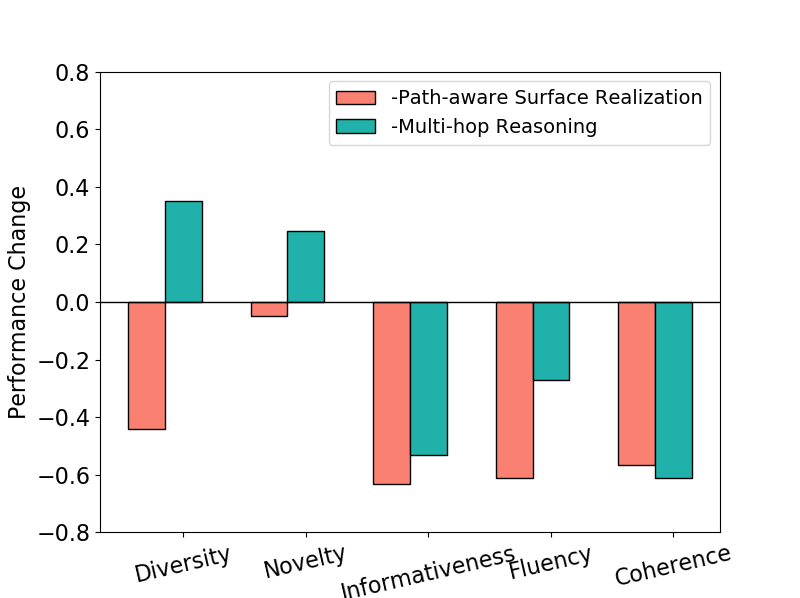
\includegraphics[width=1.0\linewidth]{ablation_study.png}
  \caption{Ablation studies of MRG-C on story generation. Diversity is measured by Dist-3, novelty is measured by Tri-Jaccard. Informativeness, fluency and coherence is measured by human evaluation on 100 randomly sampled pairs. Y-axis shows the percentage of the performance change compared  with  MRG-C. 
  \label{fig:ablation}}
  \end{figure}
  
  
\subsection{Ablation Study}
Here we conduct  ablation studies to verify the effectiveness of two modules. Figure~\ref{fig:ablation}  demonstrates the results.

% \subsubsection{Multi-hop Reasoning Ablation}
\medskip\noindent\textbf{Multi-hop Reasoning Ablation}\hspace{1em}
Specifically, in reasoning stage we replace the  multi-hop reasoning module with a random reasoning module which randomly labels 1/3 concepts as target concepts, 1/3 as intermediate concepts. As we can see from Figure~\ref{fig:ablation}, the coherence and informativeness declines significantly when the reasoning module is removed. This illustrates that the multi-hop reasoning module is crucial to generating coherent text. The multi-hop reasoning module infers skeleton paths which bridge the  preceding sentence with the following ones, and random reasoning cannot model such semantic dependencies. 
% \subsubsection{Path-aware Sentence Realization Ablation}

\medskip\noindent\textbf{Path-aware Sentence Realization Ablation}\hspace{1em}
Specifically, we only use the target concepts to generate the subsequent sentence without using the conceptual path information. As shown in Figure~\ref{fig:ablation}, when the inferred paths are replaced with the target concepts, all five indicates drop, indicating that the intermediate path information are essential for improving the quality of generated text. The inferred conceptual skeleton paths provide plenty of information which is crucial to  informative and coherent text generation.    

% Figure~\ref{fig:ablation} demonstrates the effects of the two module. When the path-aware module is ablated, all five indicators drop, indicating that conceptual reasoning paths improve the quality of generated sentences significantly. The possible reason lies in that target concept along cannot model  semantic connection among sentences. Beyond that, conceptual reasoning path provides plenty of information which is crucial to  informative, diversified and novel text generation.    
% When the reasoning module is ablated, the diversity and novelty improve, but the informativeness, coherence and fluency drop significantly, especially in terms of informativeness and coherence. 
% The reason maybe lie in that randomly selecting 1/3 concepts as target concepts and intermediate concepts contain too many noisy words which decline the coherence, informativeness and fluency but noise words can contribute to diversified and novel text generation. The ablation study shows that both the two modules play an important role in improving the effect.



% Figure 3 shows the effects of mulit-hop reasoning module on different metrics. Without multi-hop reasoning module 

% \subsubsection{without reasoning module}
% \subsection{Reasoning without a ready-made Knowledge graph}
% Knowledge  contained in  Conceptnet can be roughly categorized into commonsense knowledge. But in some situation such as e-commerce, there exists not a proper external knowledge with a good coverage with training data,  using Conceptnet as the external graph for multi-hop reasoning  will  have a litter help for long text generation. Therefore, we propose to build an Self-constructed Graph based on training data via point-wise mutual information. We propose a description generation datasets collected from Taobao \footnote{www.taobao.com} to evaluate the effectiveness of our proposed model when ConceptNet is unbefitting. This task aims at generating a long description text according to given several topic words. The proposed dataset contains 340K, 5K, 5K pairs for training, validation, test set respectively. For building an  Self-constructed Graph for this dataset, we first concatenate topic words and it's paired description as a whole example. Then, we calculate PMI between any two words appearing in vocabulary, for each word we connect those words with the most  20 great PMI value with it.  The detailed information about how the Self-constructed Graph is constructed  can be found in appendix.  


\subsection{Case Study}
Table~\ref{case} presents several examples  generated  by different systems. 
The baselines tend to generate low-quality texts in story generation. For example, texts generated by Seq2Seq and Transformer are very generic and suffer from bad inter-sentence coherence and repetition issues. Because they do not explicit model semantic dependencies among sentences. For GPT-2-FT, much of the content except for the first sentence is unrelated to the input. Besides, it suffer from repetition issues (e.g. \textit{went to beach for a day of fun}). Neither Skeleton2Seq nor GPT-2-KE can express information about keyword ``dance'' in the topic sentence. Although Plan\&Write can embody content about both keywords ``wedding'' and ``dance'', its output is relatively incoherent and less informative.
% e.g. ``the bride and groom were so happy to be married''. 
% By introducing external knowledge, Transformer-CC can generate more diversified text than vanilla Transformer. 
% However, due to without concept reasoning, the generated text lacks coherence and logic, e.g.,  ``The band played with the lead singer, the band played a trumpet player was very well.''. 
% For GPT-2, much of the content except for the first sentence is unrelated to the input. After enhanced with ConceptNet, GPT-2-KE yileds more specific topic words.
% the first few generated sentences is highly relevant with input, but as the text length grows, uncorrelated text appears, such as ``swimming'', ``play in the water'' is generated as the topic sentence is about ``Indian dance wedding'', showing long text generation is a challenging task, even the powerful pre-trained model is  discouraged in this field.  
In comparison, our methods can generate more diversified and coherent sentences with a multi-hop reasoning module to introduce external knowledge into sentence-level dependencies modeling.
% Besides, MRG-S generates more lower frequency words such as ``bridesmaids'' which doesn't exist in ConeptNet but in training data, showing how Self-constructed Graph help improve diversity on story generation. 
For a better demonstration, Figure \ref{fig:reasoningpath} presents the reasoning path, which provides an explanatory way to help understand how MRG works. 
As to product description, it can also be found that MRG reaches a better result than Seq2Seq and Transformer. Specifically, it has stronger ability in generating longer texts with abundant information. The case shows that MRG is able to provide a detailed description of the features.%, while the baselines demonstrate boring and repetitive expressions.



%%%%%%%%%%%%%%%%%%%%%%%%%%%%%%%%%%%%%%%%%%%%%%%%%\scaleboxconc
\begin{table}[!t]
\footnotesize
\small
\centering
\scalebox{0.92}{    \begin{tabular}{|p{1.00\linewidth}|}
    \hline
    %   \textbf{Input 1}: \textsl{every kind of musician was onstage.}\\
    %   \textbf{Seq2Seq}:  \textsl{she was so excited to see the organization ...[repetition]. the organization organization is always a great job. it was a great day.}    \\  
    %   \textbf{Transformer}: \textsl{the audience was very talented. the audience was very talented. the audience was very talented. the band was really good. i was so happy to be there.} \\
    % %   \textbf{Transformer}: \textsl{they love to show off their talent. they love to show off their talent. they love to show off their talent.}\\
    % %  \textbf{Transformer-K}: \textsl{they had a lot of interesting things to do . they were all very colorful . they were very colorful . they were very colorful .}\\ 
    % %  \textbf{Transformer-CC}: \textsl{the drummer was very excited . the band played with the lead singer . the band played a trumpet player was very well . the guitarist played the guitarist played his guitar player was very impressive .}\\
    % \textbf{Skeleton2Seq}: \textsl{*}\\ 
    % \textbf{GPT-2}: \textsl{the band played a lot of songs. the crowd was very excited. the family went to the beach. they saw a lot of different things. they saw a lot of different things...[repetition]}\\ 
    % \textbf{MRG-C}: \textsl{the singer was fantastic. we had a great time at the concert. at the end of the night, they listen to the band. the band played music for the night. we went home to celebrate.}\\ 
    % \textbf{Ground Truth}: \textsl{singers belted out their melodies with passion. a guitarist plucked his strings. a female vocalist lent her voice to the band. a younger lad even took to the stage, keeping up with those much older than him.}\\
   
    \textbf{Input 2}: \textsl{there was an Indian dance wedding today.}\\
      \textbf{Seq2Seq}:  \textsl{the bride and groom were very happy to be married. the bride and groom danced the night away. the bride and groom danced the night away.}    \\  
        \textbf{Transformer}: \textsl{the bride and groom exchanged vows. the bride and groom were so happy to be married. the bride and groom were so happy to be married.}\\
      \textbf{Skeleton2Seq}: \textsl{the bride and groom are happy to be married. the bride and groom are happy to be married. the wedding party is very beautiful and happy. the little family pose for a photo.}\\ 
      \textbf{Plan\&Write}: \textsl{the groom was happy to be married. the bride and groom took their first dance. then they took a picture together. they danced the night away.}\\ 
      \textbf{GPT-2-FT}: \textsl{the bride and groom were very happy. the family went to the beach for a day of fun. they had a great time. they had a great time swimming. they had a great time playing in the water. the family went to the beach for a day of fun...[repetition]}\\ 
      \textbf{GPT-2-KE}: \textsl{the bride and groom were very excited. the ceremony was held indoors. the bride and groom had a great time. the flower girl was so happy.}\\       
 
      
    \textbf{MRG}: \textsl{the bride dances with her bridesmaids. the bride and groom wore matching glasses. the bride and groom share a romantic kiss. the bride and groom exchanging vows. the bride and groom walked down the aisle.}\\ 
     \textbf{Ground Truth}: \textsl{there was a lot of dancing. the bride and groom 's first dance. it was all smiles and laughter. the whole family was there!}\\
    
    \hline%Dessert was the best part. Simple and tasty.

    % \textbf{Input 2}: \textsl{there was an indian dance wedding today.}\\
    
    
    \textbf{Input 2}: \textsl{2019 new Hepburn-style loose dress for summer, with lapels and beads, figure flattering.}\\
    %   \textbf{Seq2Seq}:  \textsl{the bride and groom were very happy to be married. the bride and groom danced the night away. the bride and groom danced the night away...[repetition]}    \\  
      \textbf{Seq2Seq}:  \textsl{This dress is designed with round collars , which helps show a pretty neck and highlights elegancy. The loose clothing pattern makes the dress comfortable to wear.}    \\
    %   \textbf{Transformer}: \textsl{the bride and groom exchanged vows . the bride and groom were so happy to be married. the bride and groom were so happy to be married...[repetition]}\\
      \textbf{Transformer}: \textsl{This dress is designed with round collars, which helps show a pretty neck and highlights elegancy. The classic round-collar design helps show a pretty neck and a pretty shape of face, and highlights elegancy.}\\
    %  \textbf{Transformer-K}: \textsl{the bride and groom were happy to be married. the bride and groom were so happy to be married. the bride and groom were so happy together.}\\
        %  \textbf{Transformer-CC}: \textsl{the bride and groom were very happy to be there. the bride and groom were very happy to be there. the bride and groom were very happy to be married. the bride and groom were very happy to be married.}\\
  %   \textbf{Template2Seq}: \textsl{The family was so happy to be there.}\\
    % \textbf{Skeleton2Seq}: \textsl{*}\\ 
    % \textbf{GPT-2}: \textsl{     the bride and groom were very happy. the family went to the beach for a day of fun. they had a great time. they had a great time swimming. they had a great time playing in the water. the family went to the beach for a day of fun...[repetition]}\\ 
    % \textbf{MRG-S}: \textsl{the bride dances with her bridesmaids. the bride and groom wore matching glasses. the bride and groom share a romantic kiss. the bride and groom exchanging vows. the bride and groom walked down the aisle.}\\ 
    \textbf{MRG}: \textsl{This dress is of a loose clothing pattern, which is suitable for most people. The design can provide you with more comforts and freedom, and the color demonstrates minimalist style. Dressing it up with a ripped pants makes you look tall and slim and demonstrates your elegancy. The fine workmanship ensures that the loose clothing pattern is casual and suitable for most figures.}\\ 
    %  \textbf{Ground Truth}: \textsl{there was a lot of dancing. the bride and groom 's first dance. it was all smiles and laughter. the whole family was there!}\\
     \textbf{Ground Truth}: \textsl{The dress with POLO collars makes you look outgoing in the photo. The beaded dress with a pair of silver pointe shoes is a perfect collocation for ladies. A simple black shoulder bag makes you look younger. The combination of sporty and debutante style is popular this year.}\\
    \hline
    \end{tabular}}
    \caption{Examples generated by the proposed approach and baselines. The top and bottom groups list the generated text on story generation and product description, respectively. The examples demonstrate that MRG can generate more coherent and informative text with less repetition in both tasks.}
    
    %The first one contains texts generated by different models on story generation, and the second one contains texts generated by models on product description generation.
   
    \label{case}
% 	\vspace{-0.10in}
\end{table}
%%%%%%%%%%%%%%%%%%%%%%%%%%%%%%%%%%%%%%%%%%%%%%%%%%%%%%

\begin{figure}[t]
\centering
\small
\footnotesize
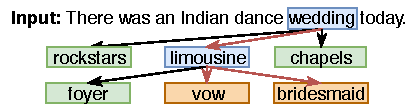
\includegraphics[width=0.9\linewidth]{reasoningpath.pdf}
% \includegraphics[\linewidth]{graph_trans.pdf}
% \vspace{-0.55in} 
\caption{An example of the inferred paths on the self-constructed graph. Blue words denote intermediate concepts. Orange words denotes target concepts. Green words denote other concepts.
\label{fig:reasoningpath}}
\end{figure}

% %%%%%%%%%%%%%%%%%%%%%%%%%%%%%%%%%%%%%%%%%%%%%%%%
% \begin{table}[t]

% \footnotesize
% \centering
%     \scalebox{0.95}{\begin{tabular}{|p{0.95\linewidth}|}
%     \hline
%       \textbf{Input 1}: \textsl{every kind of musician was on stage.}\\
%     \textbf{MRG-C Reasoning path}: musician $\rightarrow$ band $\rightarrow$ concert.\\\hline
    
%     % \textbf{Input 2}: \textsl{The lincoln museum had a lot of information about his dead.}\\
%     % \textbf{Pivot concepts}: set \\\hline
    
%     \textbf{Input 2}: \textsl{there was an indian dance wedding today.}\\
%     \textbf{MRG-I Reasoning path}:   wedding $\rightarrow$ bridesmaid, wedding $\rightarrow$  rockstars $\rightarrow$ aisle.\\\hline
%     \end{tabular}}
%     \caption{The reasoning path.} 
%     \label{reasoningpath}
%     %\vspace{-0.1in}
% \end{table}
% %%%%%%%%%%%%%%%%%%%%%%%%%%%%%%%%%%%%%%%%%%%%%%%%%


\section{Related Work}
% In the following, we provide a review of the significant previous work in both multi-hop reasoning and text generation.  
\medskip\noindent\textbf{Multi-hop Reasoning.}\hspace{1em}Multi-hop reasoning has been drawing attention in the fields of natural language processing and machine learning.
The most representative tasks are Meta QA~\citep{zhang2018variational} and PathQuestion~\citep{zhou2018interpretable} in open-domain question answering over knowledge bases and Hotpot QA~\cite{yang-et-al:hotpotqa} in reading comprehension.
Recently, researchers have conducted a series of methods for multi-hop reasoning on graphs and obtained significant performance gains~\cite{zhou2018interpretable,qiu-et-al:multihop1,DBLP:conf/emnlp/JiangB19,DBLP:conf/acl/TuWHTHZ19,ding-et-al:multihop2}. Those methods formulate multi-hop reasoning as a sequential decision problem and solve it using GNNs~\citep{gcn,gat} or Memory Networks~\citep{memoryNetworks,DBLP:conf/icml/KumarIOIBGZPS16}. In this work, we propose to perform 
sequential decision on a knowledge graph with a powerful pre-trained model BERT. In addition, our work can be seen as the first step to study how multi-hop reasoning can help long text generation.
% However,  there still exists few studies about multi-hop reasoning for text generation, especially long text generation.   

\medskip\noindent\textbf{Long Text Generation.}\hspace{1em}The most popular models for text generation are Seq2Seq~\cite{sutskever-et-al:seq2seq} 
with attention~\cite{bahdanau-et-al:attention} 
and Transformer~\cite{vaswani-et-al:transformer}. 
However, these models have limited capacity in modeling complicated semantic dependencies among sentences~\cite{wiseman-etal-2017-challenges}, often suffer from logic conflicts.
%  and lack of long range coherence  in  generated text
There are two lines of work to tackle this challenge. 
The first line attempts to model long-term semantic dependencies among sentences by a huge-size model pre-trained on a large-scale dataset~\citep{radford-et-al:gpt2,unifiedlm,mass,gpt2-ke}. These methods can be categorized into implicit semantic dependencies modeling. 
% One is the implicit modeling semantic dependencies.~\citet{radford-et-al:gpt2,unifiedlm,mass} propose a huge-size model pretrained on data of large scale, which is able to model long-term semantic dependency. 
Another line is to explicitly model semantic relationship by simplifying sentence structures, i.e., models first plan a skeleton and then expand this skeleton to a long text. ~\citet{martin-event} extracted event sequences as skeletons.
% The second line of work approximates the semantic dependencies of the entire sentence by simplifying the sentence structure and then modeling only the semantic dependencies of the sentence skeleton. 
~\citet{xu-et-al:skeleton_jingjingxu_emnlp8} adopted a reinforcement learning method to extract sentence skeletons. ~\citet{li-et-al:coarse2fine} produced a syntactic sketch with additional part-of-speech tagging tasks. ~\citet{plan-and-write}  generated a sequence of keywords as planning conditioned upon the input.
 ~\citet{long-hunag} planed input items as a sequence of groups  and then realized each sentence conditioned on the planned result and the previously generated context. Different from those models, our methods build sentence-level dependencies by inferred skeleton paths on a knowledge graph, which is more interpretative and can cover more knowledge important for 
semantic transfer.
%  and can be see as the first attempt to introduce multi-hop reasoning into long text generation filed. 
%  Besides, our methods related to use knowledge graph to generate text~\citet{knowledge-one,knowledge-two,knowledge-three,knowledge-guan}.
% This paper explores the way to model semantic dependency among sentence via multi-hop reasoning in knowledge graph.

% \citet里面尽量不要写多个，如果同一作者还可以接受  : 好的
% Our work is also related to incorporating knowledge graph into text generation \cite{minliehung_commonsense_ijcai,graphTransformer,knowledgeablestoryteller}

\medskip\noindent\textbf{Knowledge-aware Text Graph}\hspace{1em}
% Our method is also related to use knowledge graph for text generation.
Recently, it has proven effective to integrate commonsense knowledge into text generation.
~\citet{knowledge-one} employed an additional knowledge encoder to improve dialogue system. ~\cite{knowledge-three} proposed to exploit commonsense knowledge for topic-to-essay generation with a memory-augmented generator.~\citet{knowledge-guan} adopted a multi-source attention mechanism to attend commonsense knowledge for story ending generation.~\citet{gpt2-ke} incorporated commonsense knowledge into pre-trained models during fine-tuning phrases. Despite their success, those  methods only attend triple-level 
knowledge and need the decoder to perform complicated  commonsense reasoning to leverage multiple triples for reasonable text generation. In comparison, our approach adopts a separate reasoning module to integrate multiple triples into a chain-like conceptual skeleton paths. The decoder just needs to focus on  generating a fluent sentence based on the inferred paths, which is more effective.
% Different from these models, our approach infers a skeleton path from knowledge graph via a reasoning module, which 
% to help long text generation.

\section{Conclusions}
% In this paper, 
% we study how multi-hop reasoning improves long text generation and propose a 
In this paper, we propose a
novel multi-hop reasoning generation model to generate coherent and informative long text via modeling complicated semantic dependencies among sentences. We adopt a self-supervised way to construct the supervisory signals to train the new model.
% This work can be viewed as the first step towards using multi-hop reasoning for long text generation.
% This work can be viewed as the first step towards multi-hop reasoning for long text generation. 
We evaluate our model on three representative long text generation tasks, and propose to build a Self-constructed graph to make the new model applicable on tasks without appropriate artificial knowledge graphs. Automatic and human evaluation show that the new model achieves substantial improvements  over a series of state-of-the-art baselines, such as pre-trained models and knowledge-enhanced models, in terms of coherence, informativeness, and novelty. 
% Besides, our methods can generete entitiy diversity text and the reasoning path that provides a explanatory view for long text generation. 
% Besides, the analyses demonstrate that our approach can generate texts of higher diversity and novelty. 
Furthermore, the inferred paths enhance the interpretability of text generation. In the future, we will elaborate the reasoning mechanism to support controllable text generation. Besides, we will make the two modules interact with and promote each other to  avoid
error propagation. 
% in the current pipeline generation system 
% In the future work, we attempt to elaborate more reasoning mechanism. 
\bibliography{aaai21}
% \bibliographystyle{aaai21}

\clearpage
\appendix

\end{document}